\chapter{Proposed approach}
\pagestyle{fancy}
% \lhead{Proposed approach}
\label{solution}

The purpose of this chapter is to discuss how we can analyze the influence of weather over fitness habits from a software engineering perspective. A bottom-up approach will be used in the following sections, summarizing the problem statement with focus on the details that will later be modeled, describing the system architecture followed by its implementation, drawbacks and overcomes, testing and monitoring techniques we used, and finally the application's user manual. 

In terms of personal \textbf{contributions} we will give a detailed overview starting from the mobile application, then moving towards implementation details. Graphical elements such as bar or line charts were introduced into the application to facilitate a rapid understanding of underlying data models. User interface design guidelines were followed in order to provide a continuous and consistent experience for a potential user. When designing the user interface, data was brought as \textbf{efficiently} as possible to reduce waiting time. The amount of messages passing through the system, over the internet, between the weather station and the mobile application, has an upper bound of around \textbf{60} messages per second. In order to do so, cloud services were integrated. There is a directly proportional cost involved for maintaining a high rate of incoming messages. Data collected from the custom-built weather station can be \textbf{reused} in later studies, as it includes over \textbf{5000} rows of structured information regarding weather measurements. The production \textbf{costs} of 3D printed components were gradually \textbf{reduced} from the first prototype costing 48 euros, to 16 euros, and then \textbf{4} euros. 

Furthermore, arguably one of the most important contributions is the usage of \textbf{open-source electronic} components made by a small start-up from the United Kingdom, called Pimoroni. This helps the reader understand that collecting data from physical devices requires knowledge on both software, but also proper hardware parts. Additional time was spent on \textbf{hardware} component \textbf{configuration}, also adding support that was missing at that time for the newer version of Raspbian, namely Buster. A pull request was made for a \textbf{patch} on the Pimoroni's \textbf{Github} repository. Finally, the system presented in this paper runs on multiple machines spread over the internet. On the one hand, services spread on the internet can ease the development, yet, on the other hand it makes the system difficult to test, maintain, deploy and monitor.

\clearpage
The following application is intended to present a simple use-case for real-time data processing, and ease data reading through graphical elements (i.e. bar/line charts, tables). It is a mobile application built using the Ionic framework on an architecture that allows us to retrain a model in real-time. Its main features are weather monitorization, fitness habits overview, and fitness trackers statistics. 

\section{Data gathering and processing}

In Figure \ref{fig:arch_overvoew}, all the rectangles are enclosing a different part of the application, like a service or framework implementation. Doubly sided arrows describe the infrastructure entity of who is the responsibility to hold and maintain that part. For example, it is the owner's responsibility to maintain the weather monitor, while it is Google's responsibility to run the data flow pipeline. The applied testing method can be found as preceded by a check mark and we will discuss about them in the section 3.5.

\begin{figure}[!htb]
    \centering
    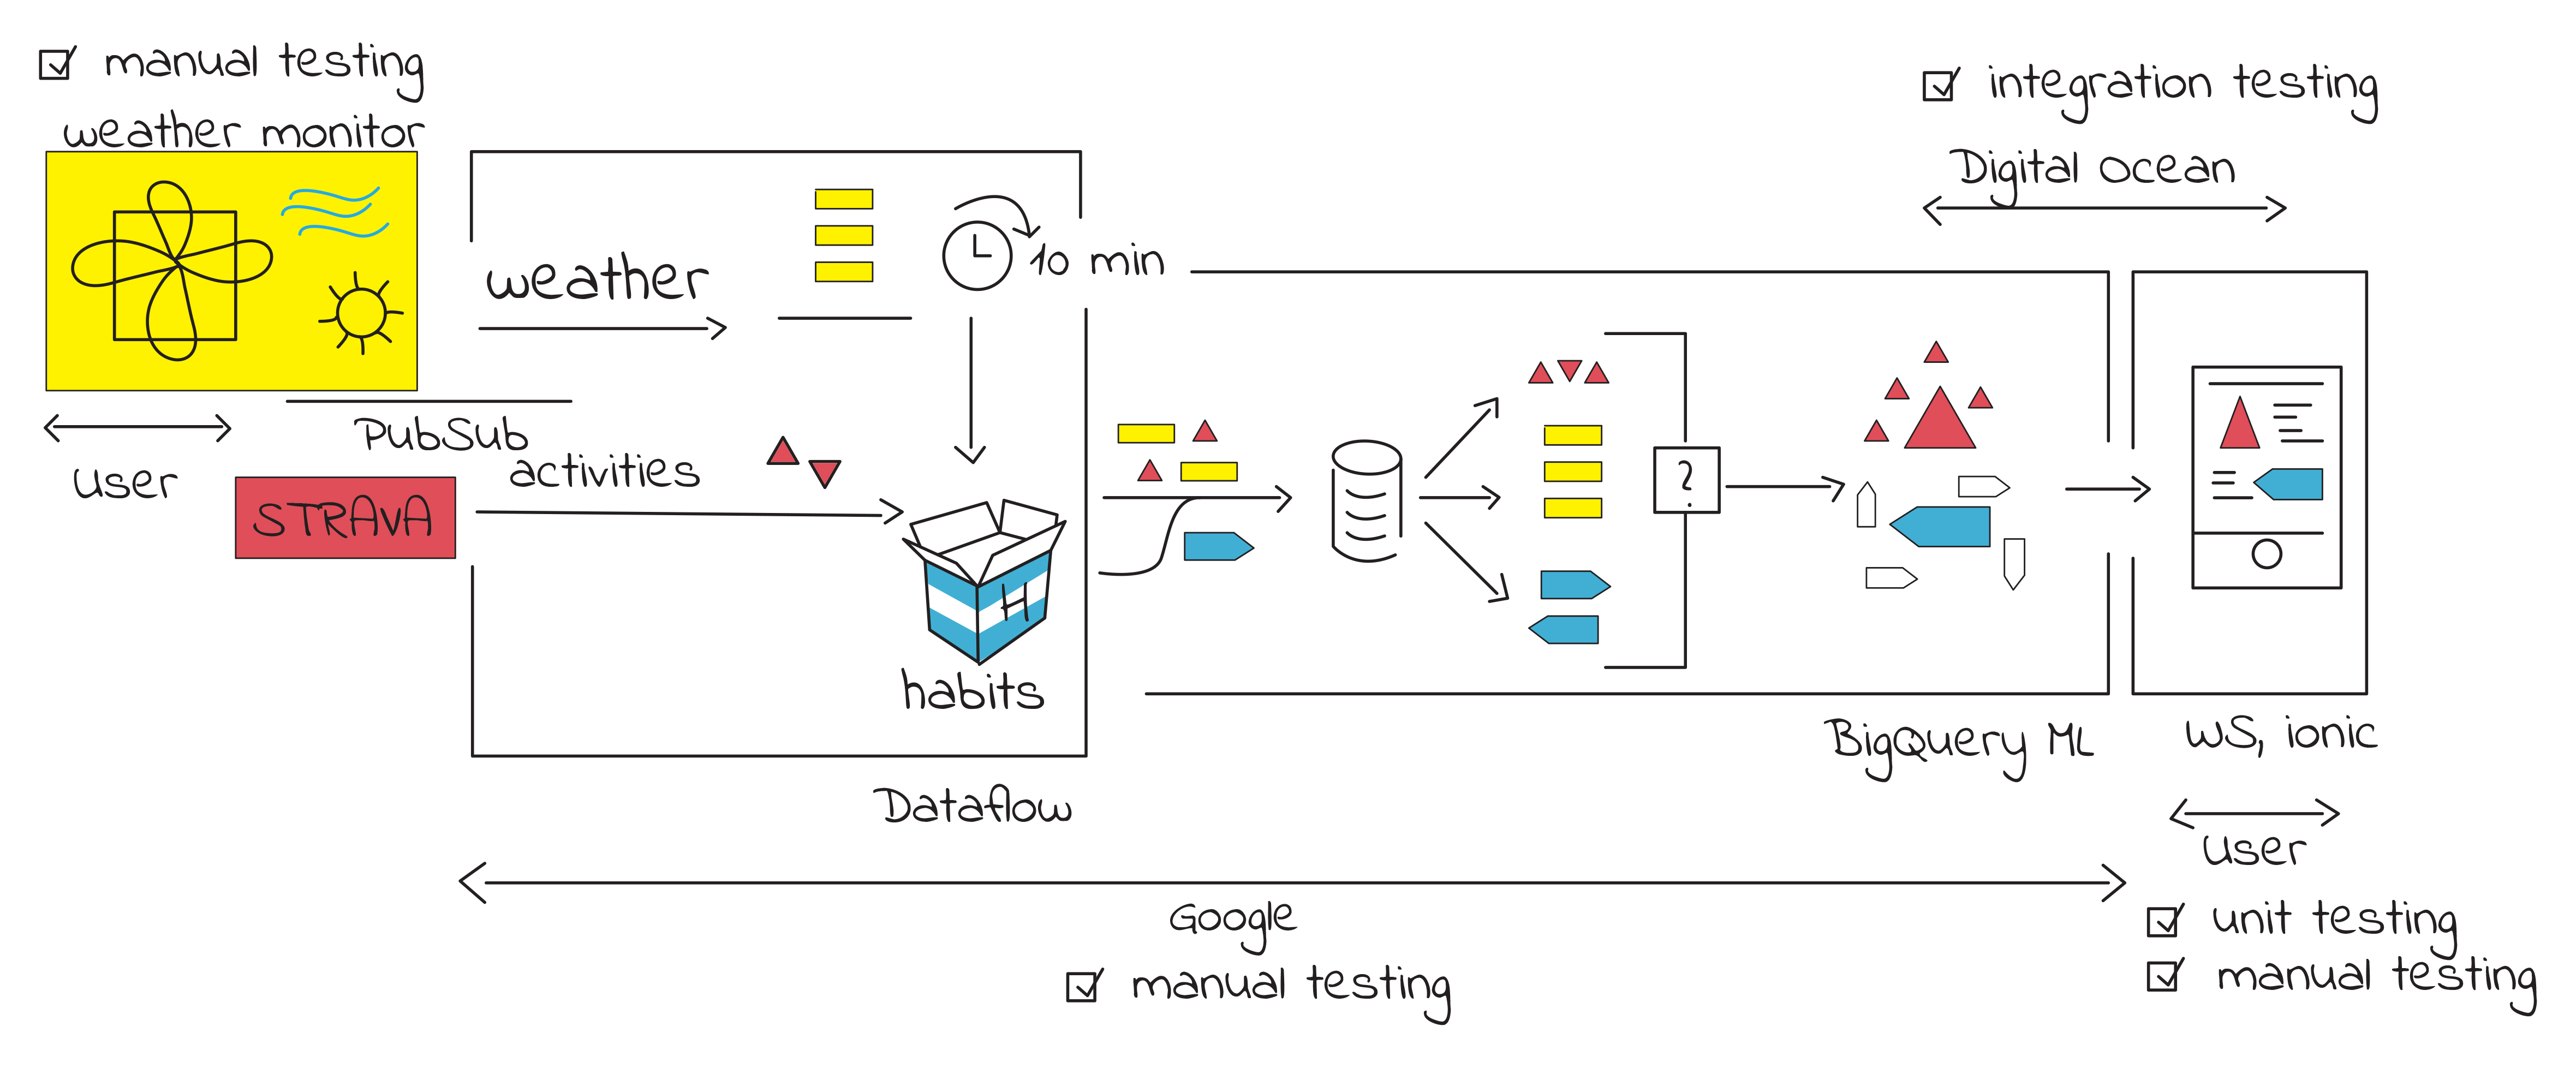
\includegraphics[width = 15.5cm]{figures/arc}
    \caption{Application overview}
    \label{fig:arch_overvoew}
\end{figure}

On the top-left corner, the yellow rectangle depicts the weather monitor. In the following table we described the data produced by taking a representative horizontal section from the persistence layer. The location column describes a geographic point in Suceava, Romania, while the color column has an RGBC format, which provides red, green, blue, and clear light sensing of lighting conditions. If the reader wishes to follow the data flow on the Figure \ref{fig:arch_overvoew}, it can find the weather measurements highlighted with yellow.

\begin{table}[!htb]
  \begin{center}
    \resizebox{\textwidth}{!}
    {\begin{tabular}{|c|c|c|*{5}{c|}}\hline
        \backslashbox[3.75cm]{Row\tnote{1}}{Attributes}
        &\makebox[3em]{\textbf{Temp.}}
        &\makebox[3em]{\textbf{Location}}
        &\makebox[3em]{\textbf{Air pr.}}
        &\makebox[3em]{\textbf{Light}}
        &\makebox[3em]{\textbf{Event time}}
        &\makebox[3em]{\textbf{Color}} \\\hline\hline
        1 & 12.7 & 47.645995 & 9707.4 & 1 & 2020-05-15 23:52:54 & 248 \\
        & & 26.252854 & & & & 335 \\
        & & & & & & 462 \\ 
        & & & & & & 1069 \\
        \hline
    \end{tabular}}
    \caption{Horizontal section through the weather measurements table}
  \end{center}
\end{table}

Strava records have a comprehensive structure when talking about their API results, yet we are interested only in a subset, so that we filtered the records and made the following structure available. They are brought to the system whenever new data was found, at specific intervals of time (i.e. 10 min). If the reader wishes to follow the data flow on the Figure \ref{fig:arch_overvoew}, it can find the weather measurements highlighted with red.

\begin{table}[!htb]
  \begin{center}
    \resizebox{\textwidth}{!}
    {\begin{tabular}{|c|*{5}{c|}}\hline
        \backslashbox[3.75cm]{Row\tnote{1}}{Attributes}
        &\makebox[3em]{\textbf{Athlete Id}}&\makebox[3em]{\textbf{Device Name}}&\makebox[3em]{\textbf{Max Speed}}&\makebox[3em]{\textbf{Total photo count}}\\\hline\hline
        1 & 13703943 & Strava Android App & 2.7 & 1 \\
        & \textbf{Athlete Count} & \textbf{Kudos Count} & \textbf{Start LatLng} & \textbf{Type} \\
        & 1 & 12 & 47.645995 & Walk \\
        & & & 26.252854 & \\
        & \textbf{Timezone} & \textbf{Elev high} & \textbf{Total elevation gain} & \textbf{Start date} \\
        & GMT+02:00 & 362.7 & 2.9 & 2020-05-07 17:50:58 \\
        & \textbf{Name} & \textbf{Elev low} & \textbf{Average speed} & \textbf{Elapsed time} \\
        & Evening Walk & 359.4 & 0.838 & 1094 \\
        & \textbf{Calories} & \textbf{End LatLng} & \textbf{Moving time} & \textbf{Distance} \\
        & 83.8 & 47.65 & 914 & 766.3 \\
        & & & 26.252854 & \\
        \hline
    \end{tabular}}
    \caption{Horizontal section through the user activities table}
  \end{center}
\end{table}

Joining the weather features with each new activity fetched from Strava gives us a habbit tuple. These tuples are used to predict the temperature, light and air pressure at which a user will be most probably comfortable, for example, to run, the next time when it engages in an outdoor activity. If the reader wishes to follow the data flow on the Figure \ref{fig:arch_overvoew}, it can find the weather measurements highlighted with blue.

\begin{table}[!htb]
  \begin{center}
    \resizebox{\textwidth}{!}
    {\begin{tabular}{|c|*{5}{c|}}\hline
        \backslashbox[3.75cm]{Row\tnote{1}}{Attributes}
        &\makebox[3em]{\textbf{Athlete Id}}&\makebox[3em]{\textbf{Avg. Temp.}}&\makebox[3em]{\textbf{Avg. Air Pres.}}&\makebox[3em]{\textbf{Avg. light}}\\\hline\hline
        1 & 13703943 & 16.53 & 9751.7 & 900.0 \\
        & \textbf{Type} & \textbf{Average speed} & \textbf{Elapsed time} & \textbf{Max Speed} \\
        & Run & 2.344 & 1799 & 7.6 \\
        & \textbf{Start date} & \textbf{Moving time} & \textbf{Calories} & \textbf{Distance} \\
        & 2018-05-12 05:27:32 & 1731 & 444.9 & 4056.9 \\
        \hline
    \end{tabular}}
    \caption{Horizontal section through the habits table}
  \end{center}
\end{table}

With those in mind, we reached the question mark, depicted in Figure \ref{fig:arch_overvoew} inside a square. At that point we are focusing on two things - finding the desired knowledge and make this process available in real-time. When we are using Cloud BigQuery ML, we create a model and with that model we are searching for patterns. Whenever new data comes into the system, that model gets retrained. During the training process, the old model remains available. After completion, the new model replaces the old one. This helps us understand how this process of pattern finding can be approached for particular instances that require data to be analyzed on the go. Represented as geometric figures significantly larger in size, the knowledge is obtained and transmitted to the application. At this moment comes in hand to use web-sockets to notify the user about changes in the business layer.

\section{Architecture design}

The system architecture is divided into four layers: IoT Data Sensing Layer, Data Analysis and Reasoning Layer, and User Application Layer. The center piece is taken by Google services, being one of the main contributions for this project - building the software solution on top of large scale services. On the left side we can see the same building blocks as in the last drawing, yet the right side describes some new technologies. Digital ocean offers ready-to-use machines running a wide variety of operating systems directly in cloud, with no operations involved in the process of development. For this project we are using a Ubuntu 18.04.3 (LTS) x64, 1 vCPUs 1GB / 25GB Disk, at (\$5/month). It was used to have the servers available over the internet. The Ionic framework made possible to integrate web components in a mobile application, as it takes an Angular project and builds the corresponding native version with one command. This drawing schematics is how we envisioned the application before knowing how to code it, yet the reader can not see the traces of erasure. They would give a hint with regard to how complicated an architecture like this might be to design so that it really works. Figure \ref{fig:system_achitecture_diagram} is more appropriate for a better understanding of the architectural components.

\begin{figure}[!htb]
    \centering
    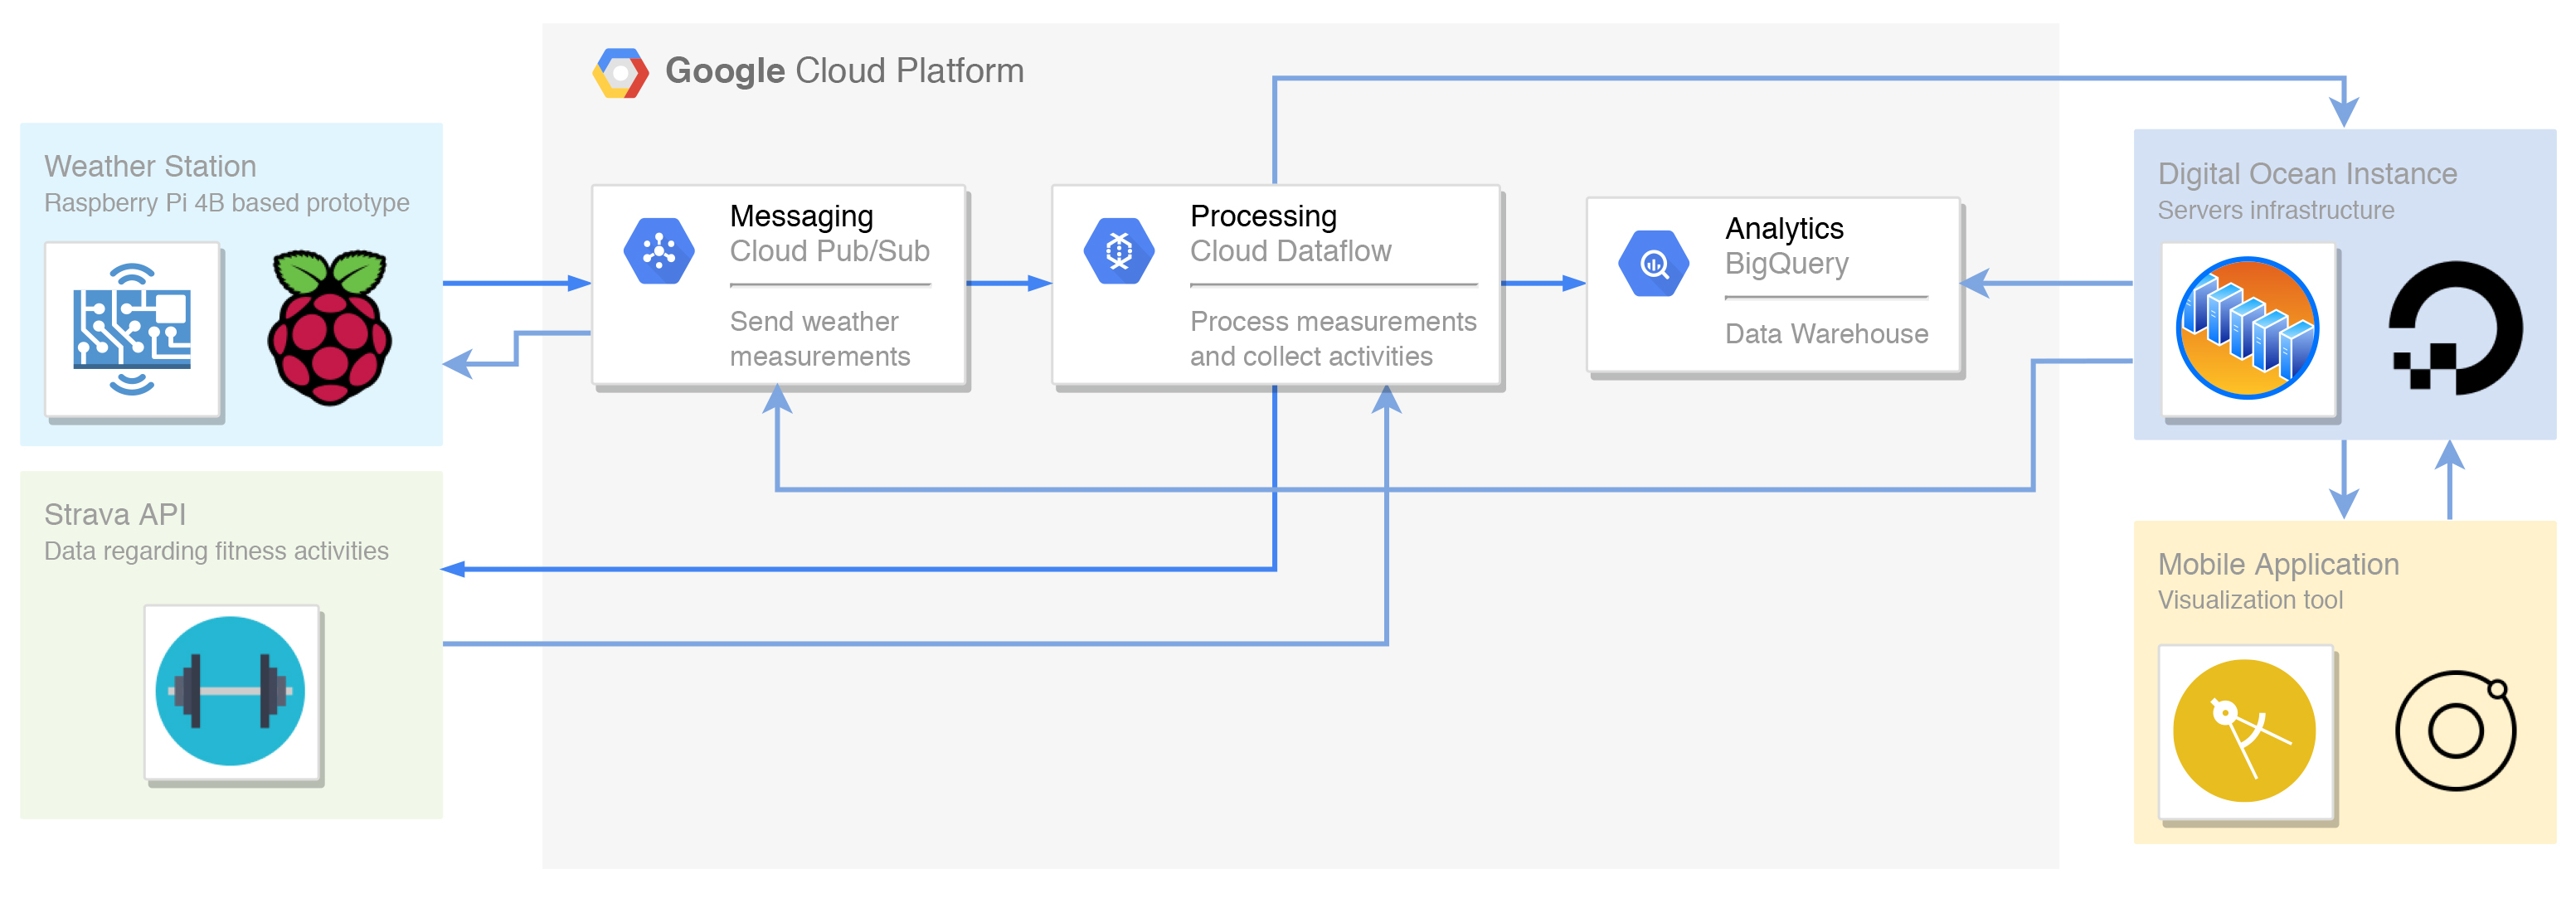
\includegraphics[width = 15.5cm]{figures/arch}
    \caption{System architecture}
    \label{fig:system_achitecture_diagram}
\end{figure}

In Figure \ref{fig:app_flow1997} three colors describe the three processes that can be considered, without a doubt, the most interesting aspects. They involve eight entities, controlling the flow. For convenience the following notations were made: WS stands for a server that makes us of the web socket protocol to facilitate data communication, while H represents a server using the HTTP protocol. Shall we start with the left side, the processes highlighted with blue illustrates data transmission between the monitor and the mobile device. Otherwise, underneath it, is described the process of sending a change display command, highlighted with red. The dataflow pipeline, the persistance layer and the computational power of the distributed system are primary building blocks for the process highlighted with purple. While PubSub facilitates transport of messages between machines, these messages are overseen by Dataflow - composing the data streaming solution we used. Windowing data is a technique of grouping messages based their timestamps. This helps us reduce the number of write operations we perform on the persistence layer. At each end of a window we fetch updates, if any, from Strava, create the habits, insert the activities, retrain the models predicting the ideal temperature, air pressure and light for fitness activities, and finally update the existing views. After the process completes, if new activities were brought from Strava, a notification will be dispatched towards the mobile application. The backend server would log the following if a new activity was fetched from Strava:

\begin{lstlisting}
Log: Fetch recent activities from Strava
2020-06-06 21:12:09+00:00
Fetched 1, the latests is on 2020-06-08 05:57:00+00:00
Log: 1 new activities.
[]
[]
Log: Model retraining..
Log: Views update..
35.223.66.107 - - [08/Jun/2020 06:18:38] "GET /bqml-retrain HTTP/1.1" 200 -
\end{lstlisting}

If no activities were discovered at the end of a time window, the following log messages will be displayed on the backend server:

\begin{lstlisting}
Log: Fetch recent activities from Strava
2020-06-08 05:57:00+00:00
empty list
Log: 0 new activities - update/retraining postponed
35.223.66.107 - - [08/Jun/2020 06:37:11] "GET /bqml-retrain HTTP/1.1" 200
\end{lstlisting}

\begin{figure}[!htb]
    \centering
    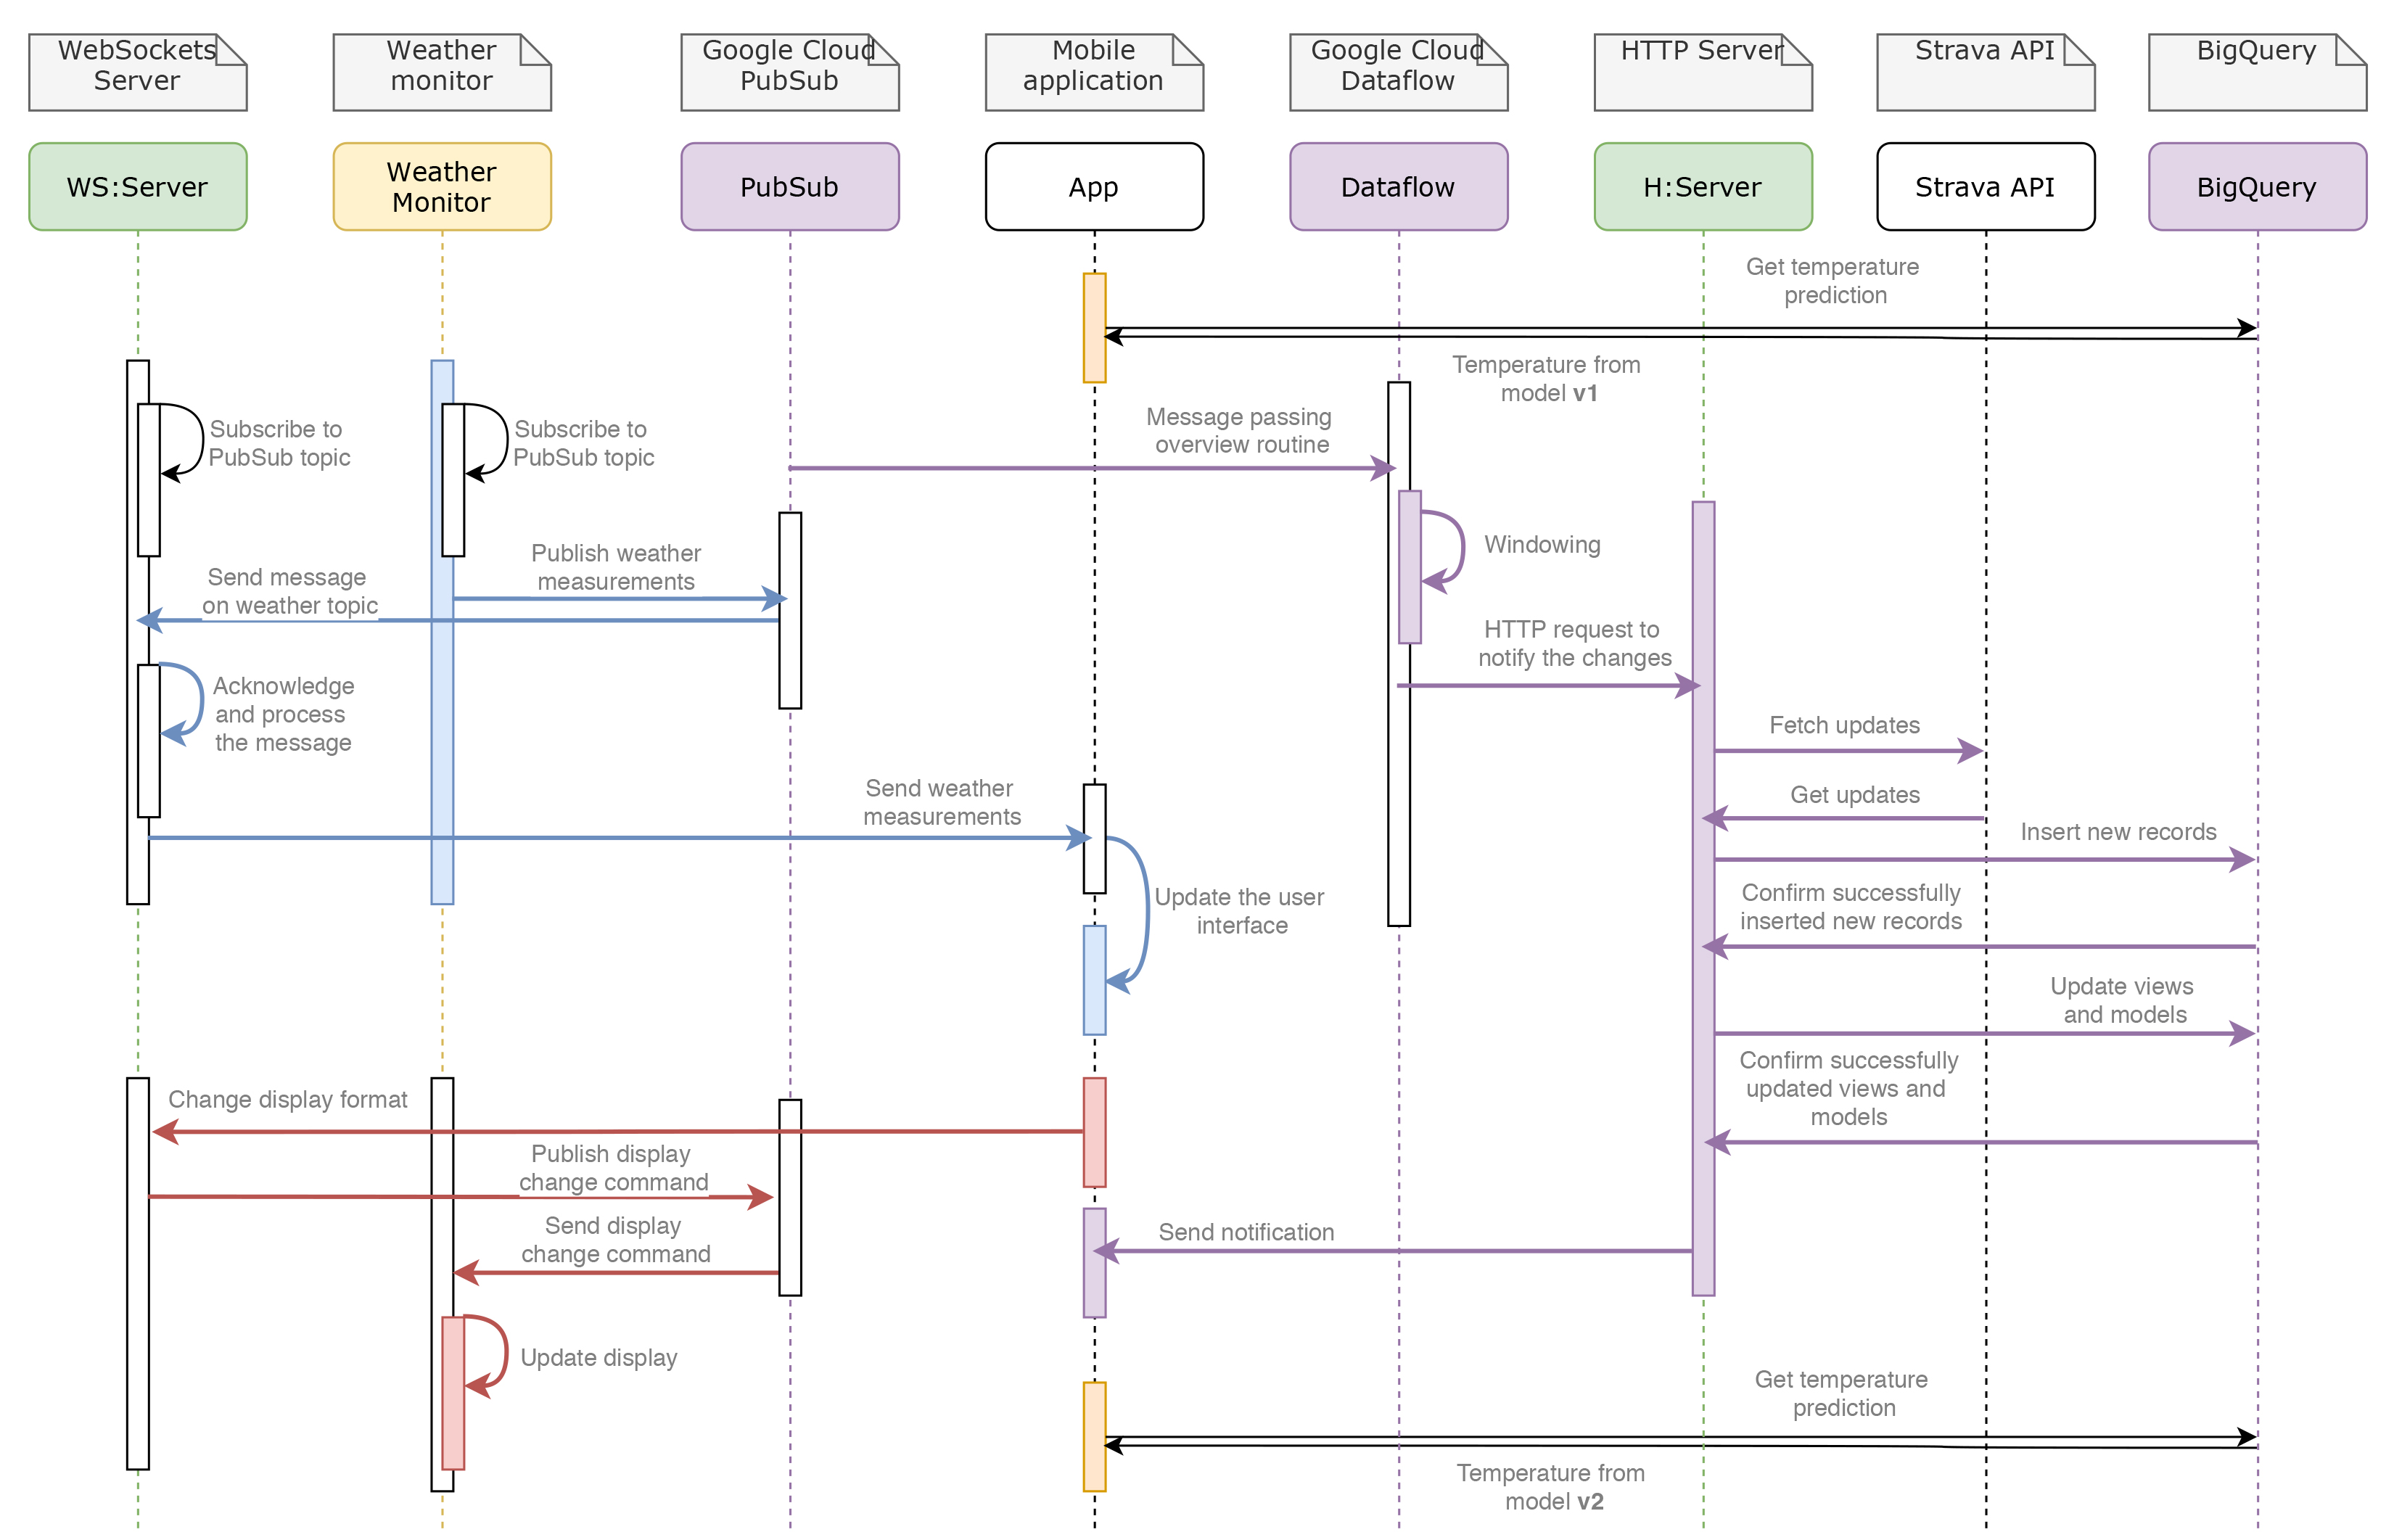
\includegraphics[width = 15.5cm]{bachelor/figures/architecture_flow}
    \caption{Application flow diagram}
    \label{fig:app_flow1997}
\end{figure}

All the actions previously described were modeled using either resources following REST standards, Apache Beam traditional transformations and par-do operations, and traditional classes which can be found in the Figure \ref{fig:backend_classes09}.

\begin{figure}[!htb]
    \centering
    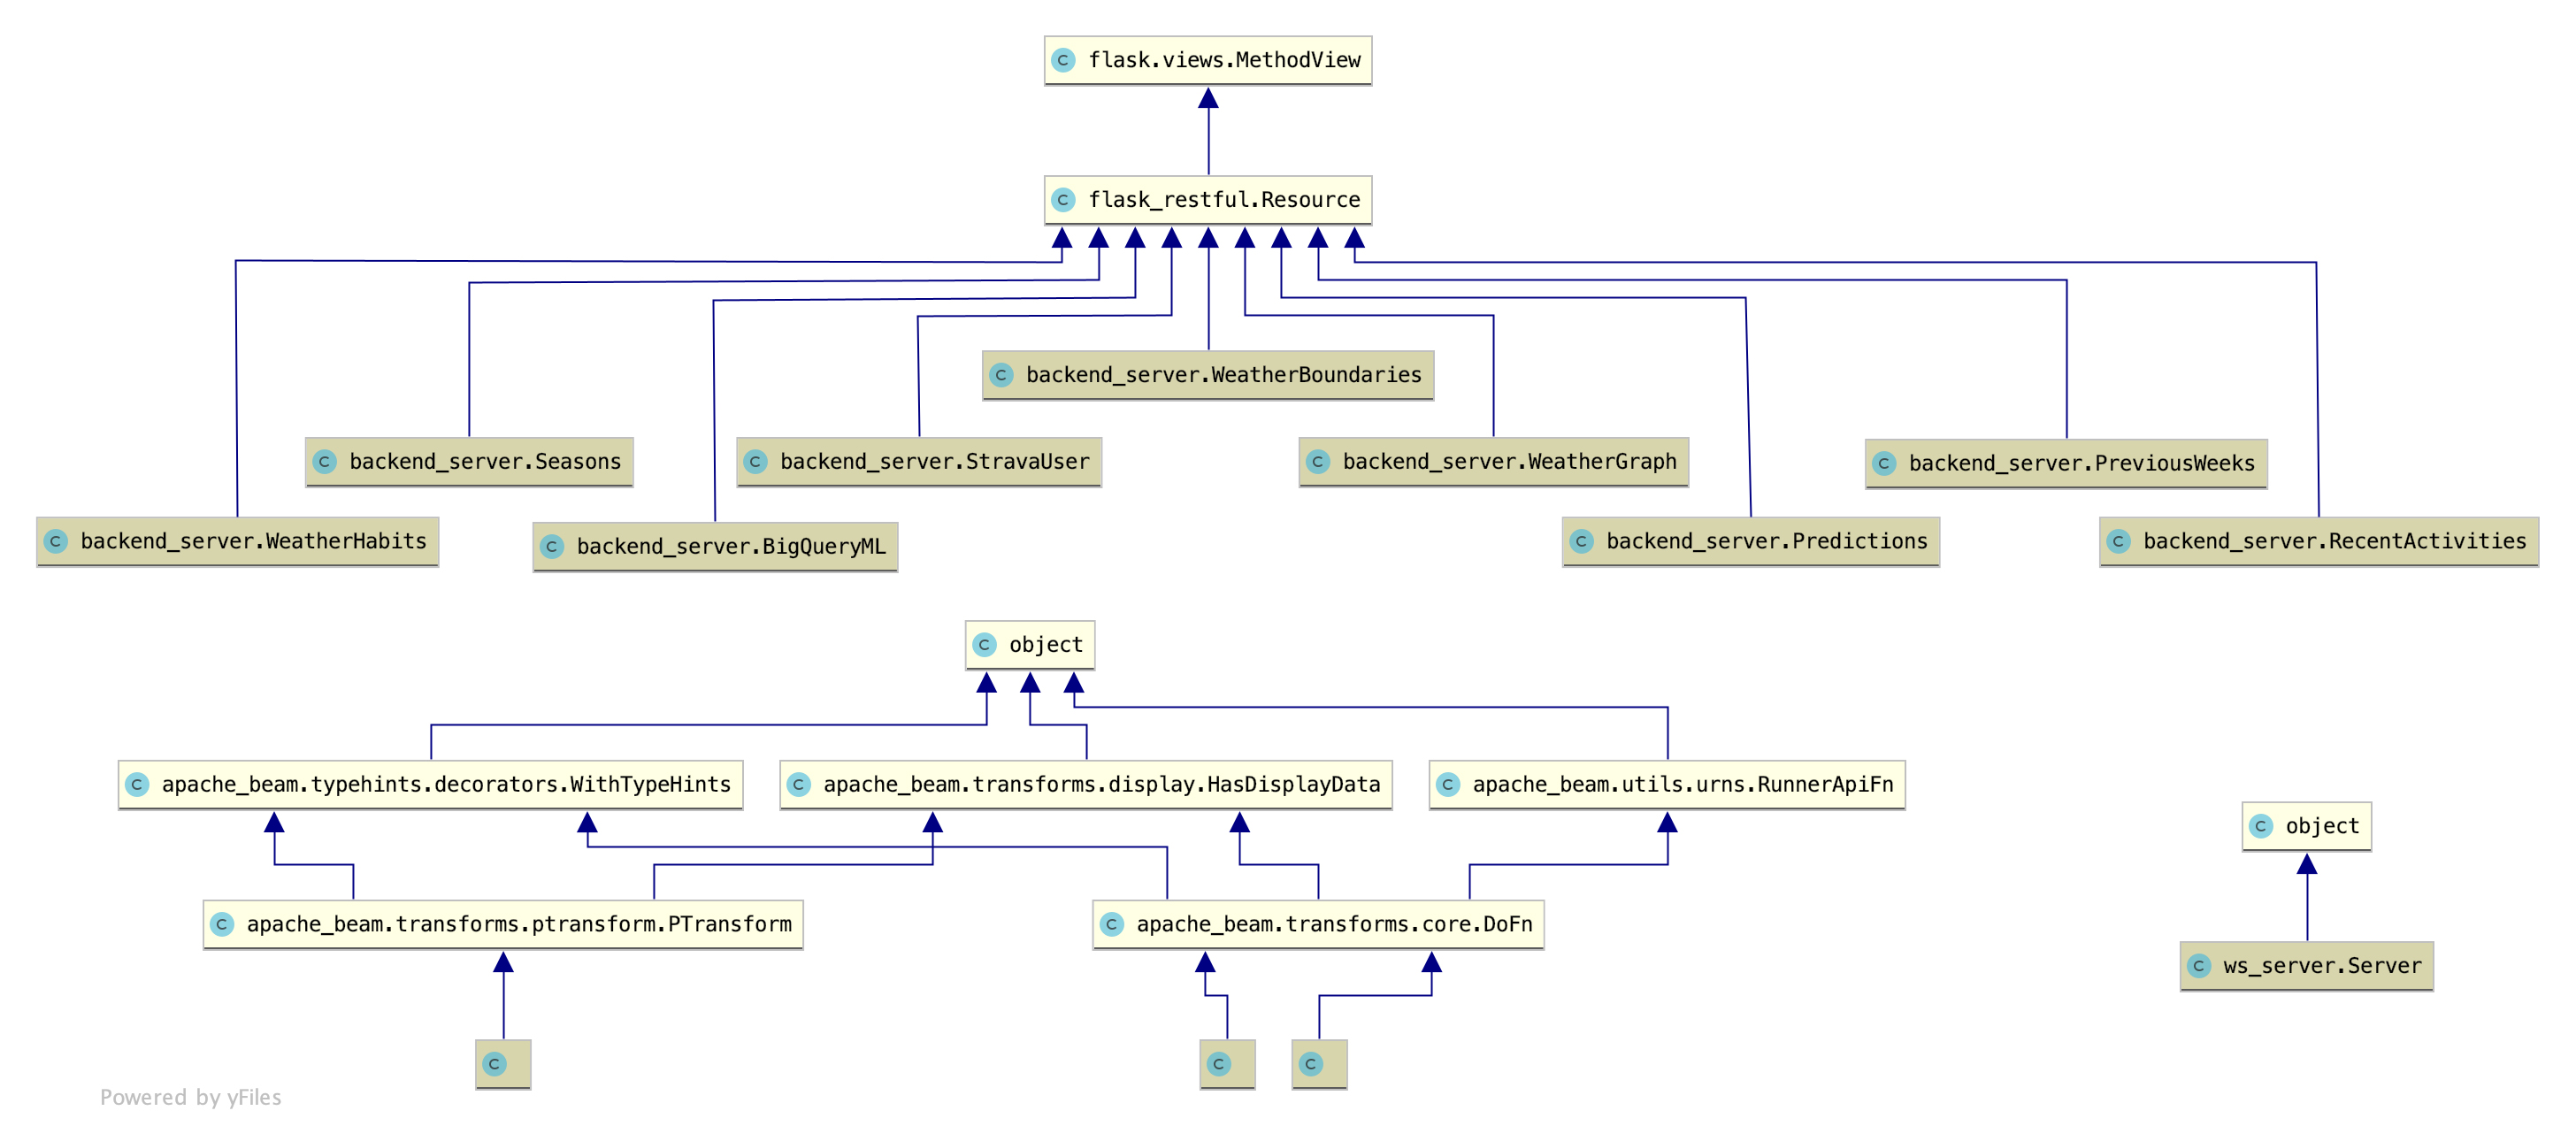
\includegraphics[width = 15.5cm]{figures/backend_cd}
    \caption{Business layer Class Hierarchy}
    \label{fig:backend_classes09}
\end{figure}

The persistence layer is composed out of four tables storing entities, well known at this point, alongside the models and views used in the business layer. One notable aspect of the storage facility is that it supports both batch and streaming I/O\footnote{Input/Output} operations.

\begin{figure}[!htb]
    \centering
    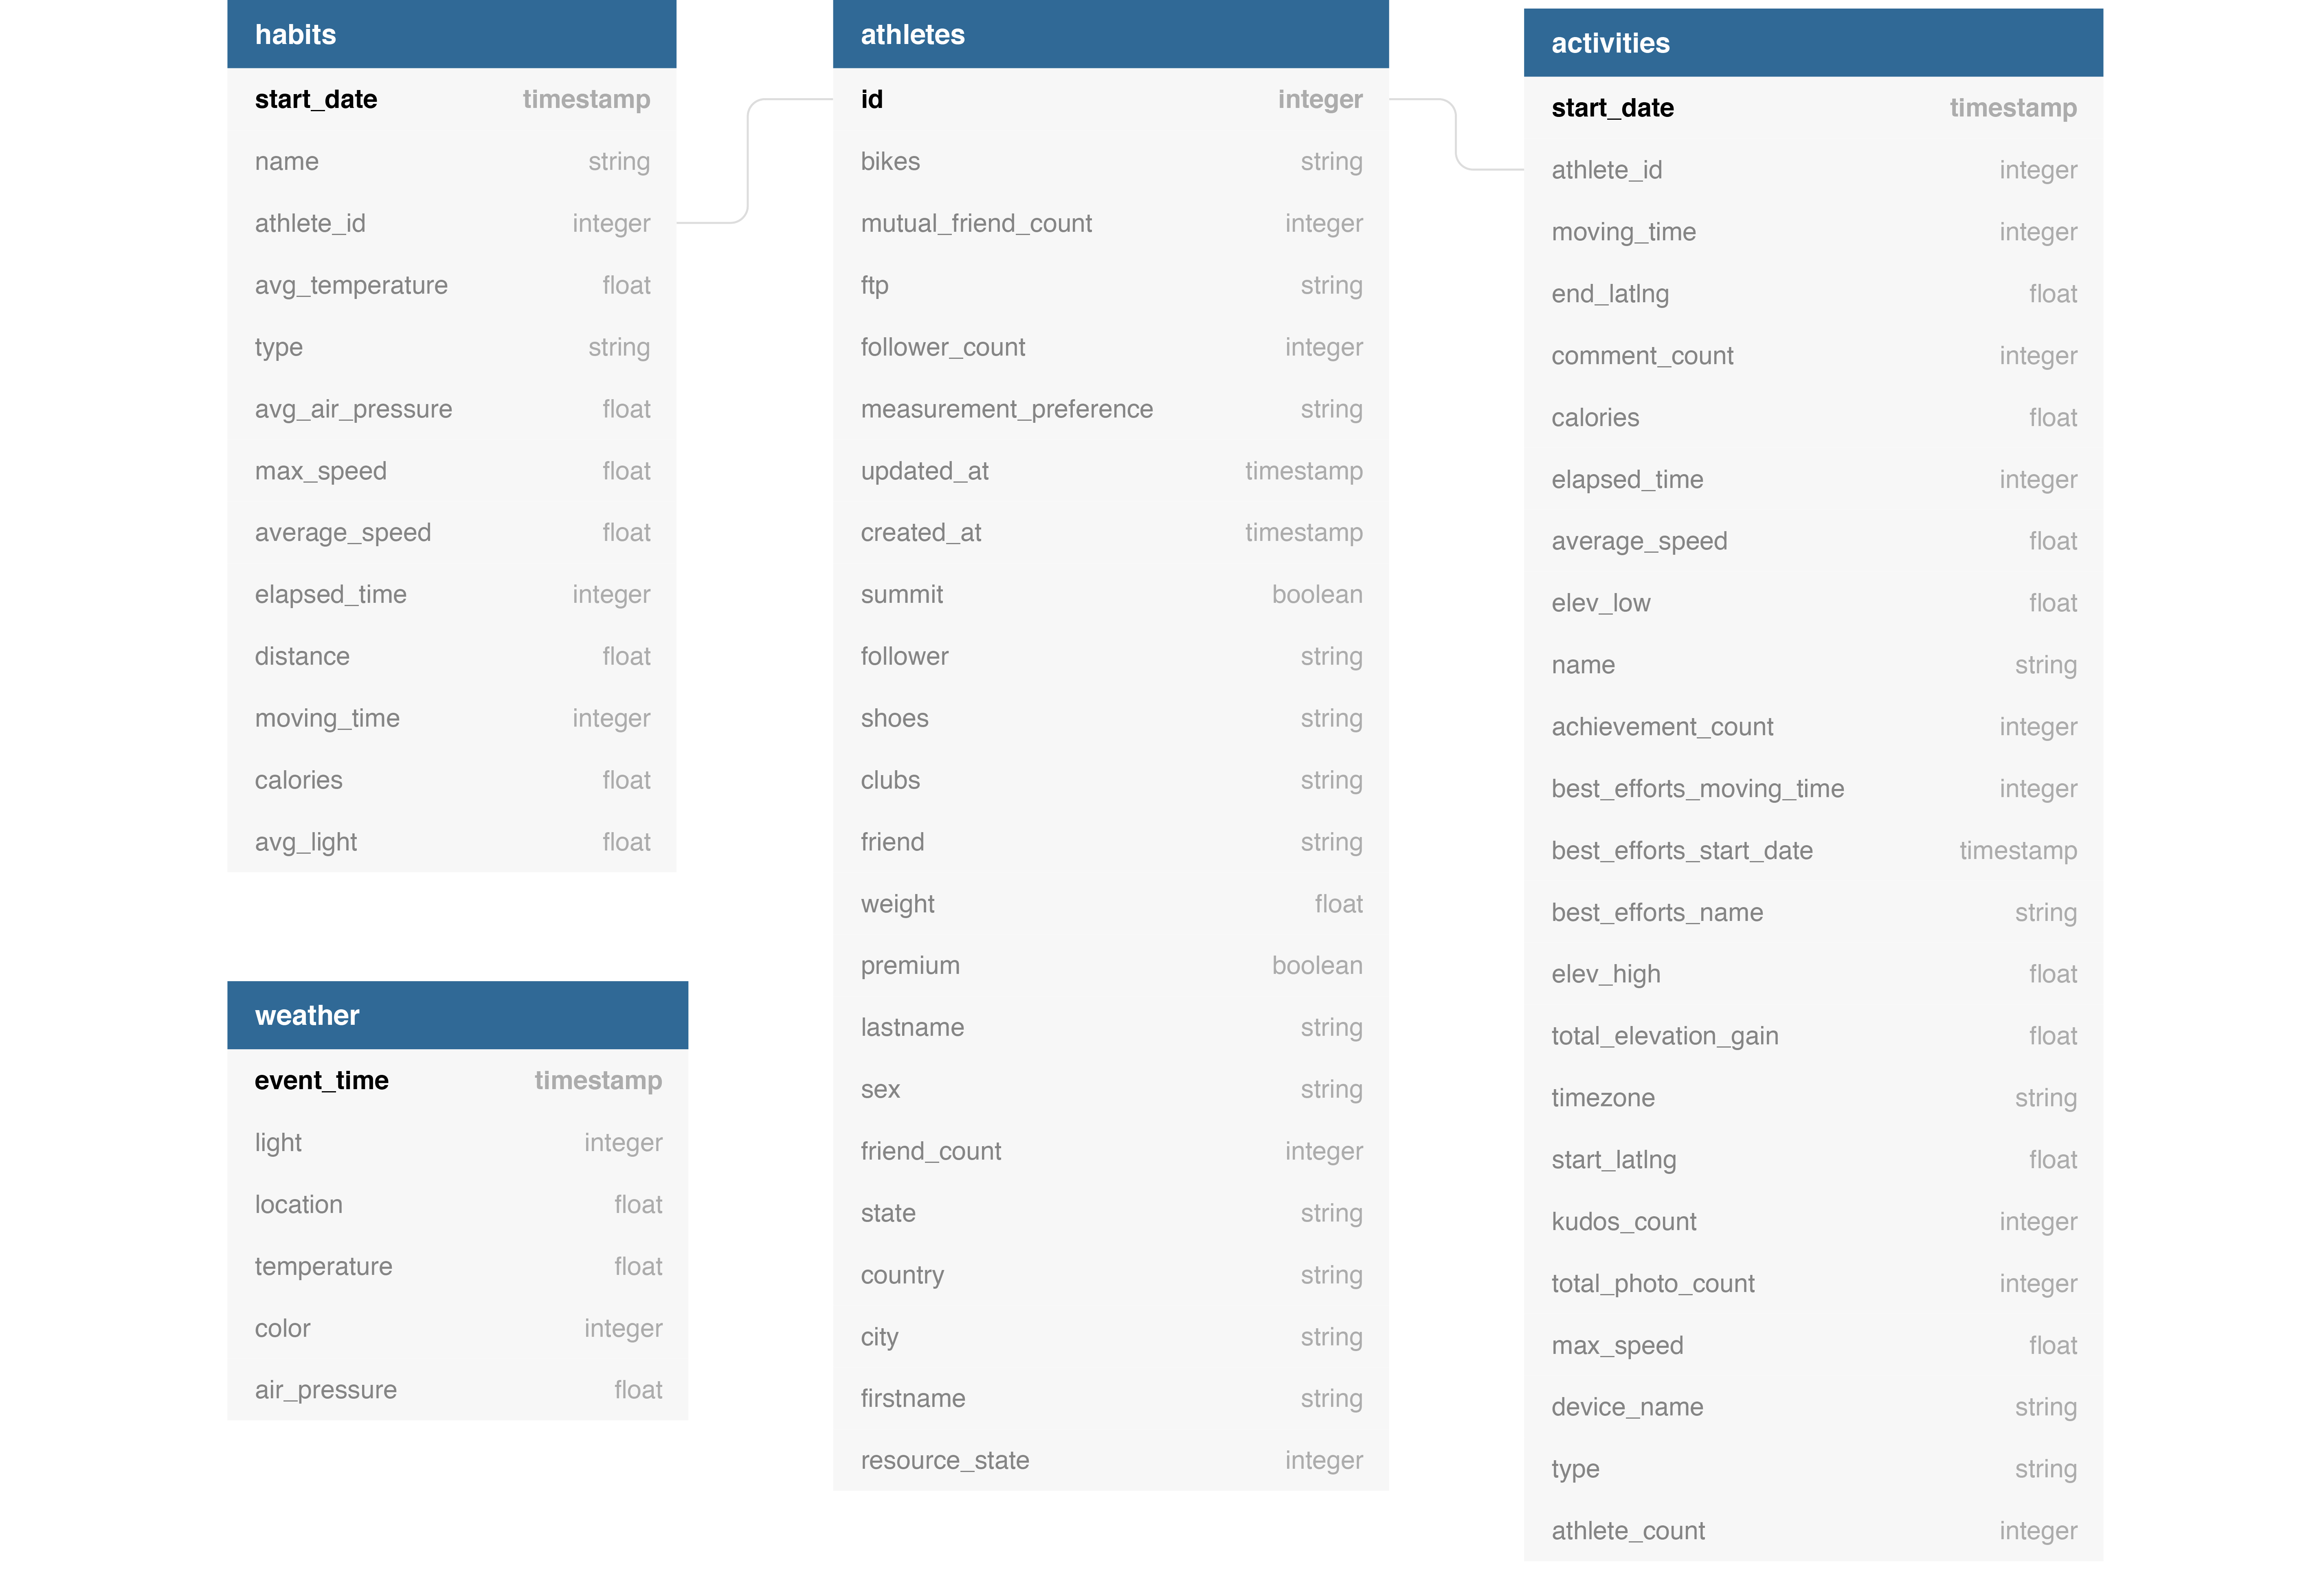
\includegraphics[width = 15.5cm]{figures/dbcd}
    \caption{Persistence layer}
    \label{fig:usecases}
\end{figure}

The mobile application has two services, one oriented towards data communication and one for local storage, a root layer for all the panels and the content of those as separate pages. 

\begin{figure}[htp]
    \centering
    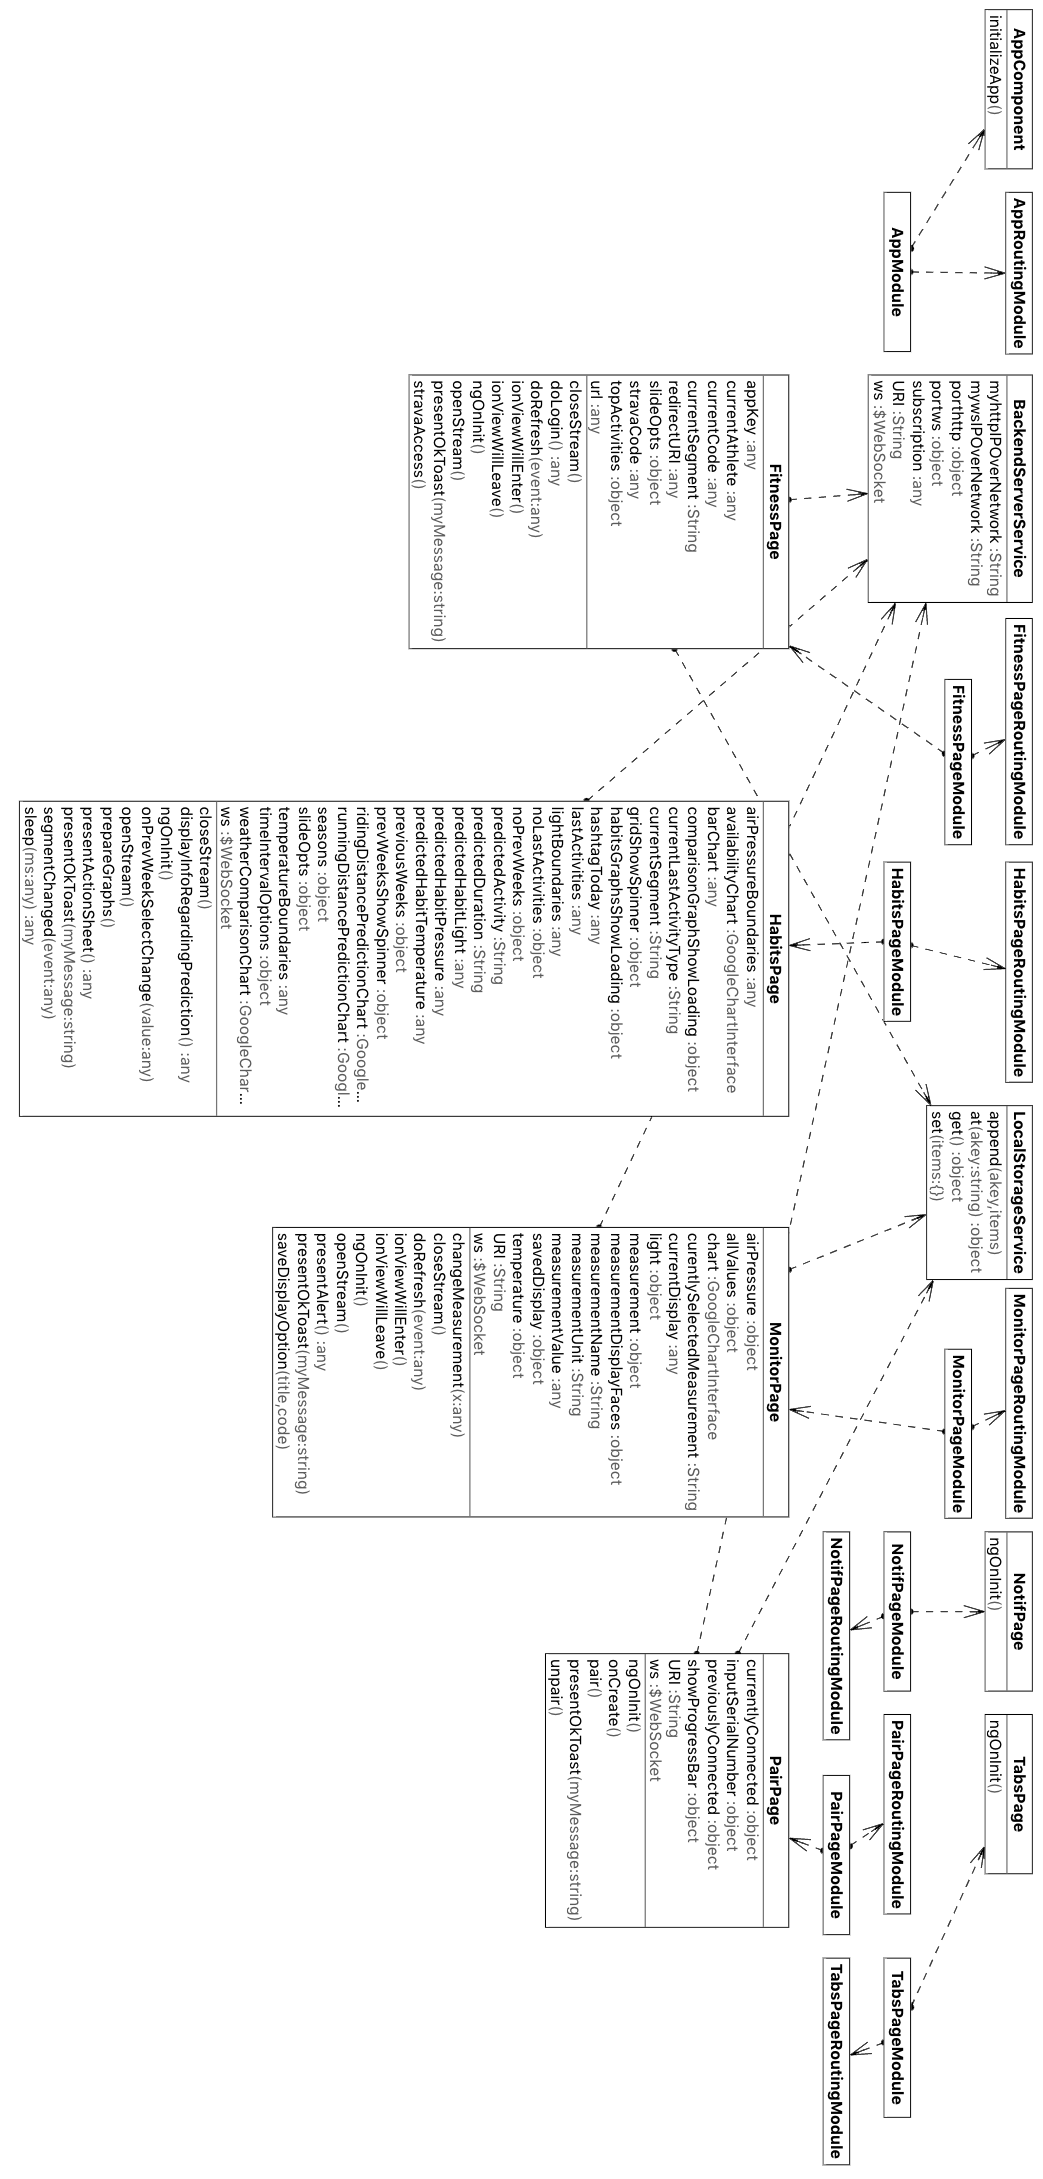
\includegraphics[width=10cm,height=23.8385cm]{figures/macd}
    \caption{Mobile application class diagram}
    \label{fig:maclassdiagram}
\end{figure}

\clearpage
\subsection{System specifications}

A hybrid approach will describe both the functional specifications and the implementation details, as we found easier to create a comprehensive bird-eye view for the reader, reducing the information seek time. In other words, if the reader finds an interesting aspect, we wanted it to immediately connect an idea to its top-down implementation. The absence of a flow diagram means that it is similar to one of the other points previously described, or it is not bringing any value to the current state of the project to describe it in more details. For example, the visual feedback of the weather indicators was implemented and manually tested on the weather device, making it less important to be described in this section than the rest of use cases.

\begin{figure}[!htb]
    \centering
    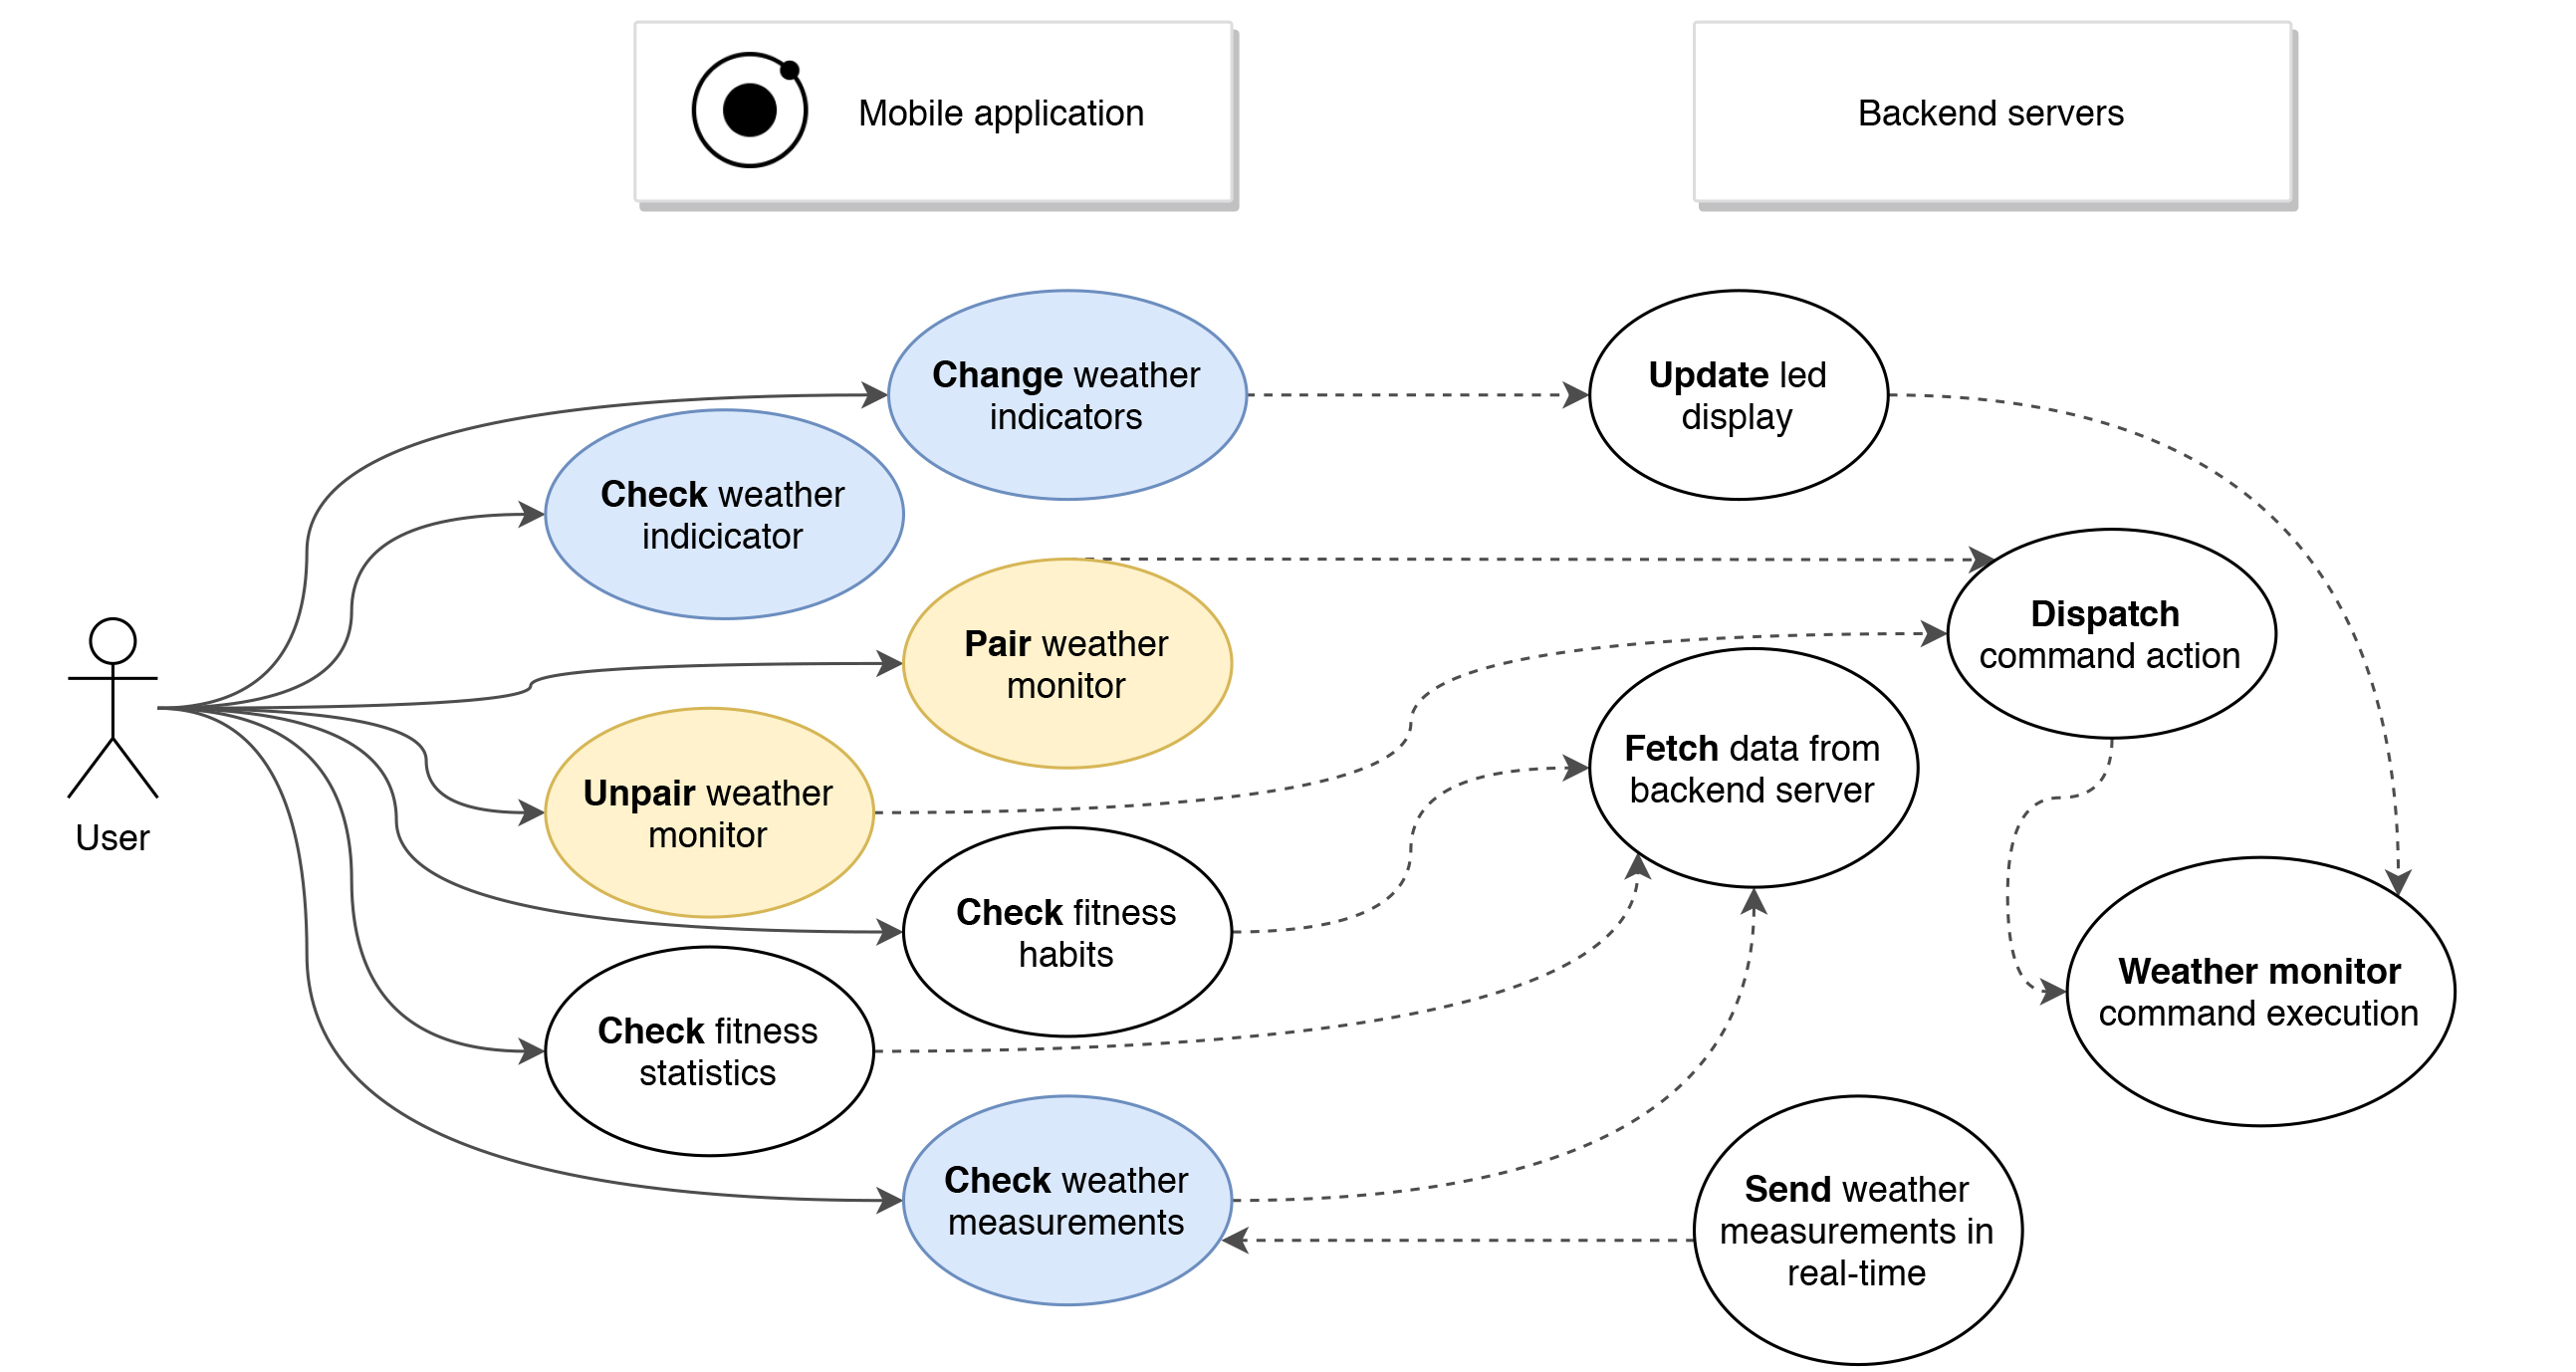
\includegraphics[width = 15.5cm]{figures/ucd}
    \caption{Application use-cases}
    \label{fig:usecases}
\end{figure}

\vspace{4mm}
\textbf{1. Visually check weather indicators}
\vspace{4mm}

This use case was manually tested through visual confirmation of the desired action.

\begin{table}[!htb]
  \begin{center}
    \label{tab:table90}
    {\begin{tabular}{p{5cm} p{12cm}}
        \textbf{Use case specifications} & \textbf{Description}\\
         Goal & \textbullet \hspace{1mm} offers a visual representation of data measurements \\ 
         & on a led based display\vspace{2mm} \\
         Pre-condition & \textbullet \hspace{1mm} the weather station should be powered on \vspace{2mm}  \\
         Post-condition & None \vspace{2mm} \\
         Constraints/Issues/Risks & \textbullet \hspace{1mm} direct exposure to high intensity light sources may \\
         & reduce the contrast and implicitly will make the\\
         & digits difficult to see\vspace{2mm} \\
          Trigger Event(s) & \textbullet \hspace{1mm} the user should select a display option \vspace{2mm} \\
    \end{tabular}}
  \end{center}
\end{table}

\begin{table}[!htb]
  \begin{center}
    \label{tab:table90}
    {\begin{tabular}{p{5cm} p{12cm}}
         System Event(s) & None \vspace{2mm} \\
         Primary Actor & \textbullet \hspace{1mm} weather station owner\\
    \end{tabular}}
  \end{center}
\end{table}

\textbf{2. Change displayed weather indicators}
\vspace{4mm}

The weather station offers a variety of display options, so that anyone with access to the physical device can check the weather measurements directly.

\begin{table}[!htb]
  \begin{center}
    \label{tab:table90}
    {\begin{tabular}{p{5.5cm} p{13cm}}
        \textbf{Use case specifications} & \textbf{Description}\\
         Goal & \textbullet \hspace{1mm} produce a visual feedback on the weather station, \\
         & changing the meaning of data displayed.\vspace{2mm} \\
         Pre-condition & \textbullet \hspace{1mm}  the weather station should be powered on and paired \\
          & to the mobile app \\
          & \textbullet \hspace{1mm} the mobile device should have a consistent internet \\
          & connection\vspace{2mm}\\
         Post-condition & None \vspace{2mm} \\
         Constraints / Issues / Risks & \textbullet \hspace{1mm} the weather station can enter an undefined state due \\ 
          & to a hardware issue\vspace{2mm} \\
         Trigger Event(s) & \textbullet \hspace{1mm} in order to preform a display update, an user must \\
         & select one of the available options that are accessible & 
         & from the "Monitor" tab, under the chart\vspace{2mm} \\
         System Event(s) & \textbullet \hspace{1mm} a message is sent from the mobile app to the weather \\
         & device \vspace{2mm} \\
         Primary Actor & \textbullet \hspace{1mm} the user which owns the weather station\\
    \end{tabular}}
  \end{center}
\end{table}

In the code listings \ref{change_weather_indicators_top} to \ref{aladinfermecat}, a couple of endpoints exchange messages between them. In the following code snippets one can better understand the implementation behind this use case.

\begin{lstlisting}[language=JavaScript, caption=User Application Layer (Ionic Application - Monitor Page), label=change_weather_indicators_top]
this.backend.ws.send(JSON.stringify({displayCode: code}))
.subscribe(
  (msg) => { ... },
  (msg) => {
      if (msg.includes('Socket connection has been closed')) {
        this.presentOkToast('Weather device cannot be reached');
      } else {
        this.presentOkToast('Cannot connect to weather device');
      }
  },
  () => { ... }
);
\end{lstlisting}

\begin{lstlisting}[language=Python, caption=Reasoning Layer (Digital Ocean instance running 'ws\_consumer.py'), label=change_weather_indicators_reasoning]
async def consumer_handler(websocket):
    async for message in websocket:
        if 'displayCode' in message:
            message = json.loads(message)
            data = "{\"displayCode\": " + 
                    str(message["displayCode"]) + "}"
            data = data.encode('utf-8')
            future = publisher.publish(topic_path, data=data)
            print(future.result())
        ...
\end{lstlisting}

\begin{lstlisting}[language=Python, caption=IoT Data Sensing Layer: 1 (Raspberry Pi running 'weather\_monitor.py')]
def display_settings():
    subscriber = pubsub_v1.SubscriberClient()
    subscription_path = subscriber.subscription_path(
        '<project>', '<subscription-topic>')
    future = subscriber.subscribe(subscription_path, 
        callback = display_settings_callback)
    t = threading.currentThread()
    while getattr(t, 'do_run', True):
        try: future.result(timeout=5)
        except Exception as exc:
            print('Timeout refresh: ', exc)
    future.cancel()
\end{lstlisting}

\begin{lstlisting}[language=Python, caption=IoT Data Sensing Layer: 2 (Open a new thread for light display execution sequence)]
def display_settings_callback(message):
    data = message.data.decode('utf-8')
    data = json.loads(data); display = False
    if display_thread is not None:
        display_thread.join()
    display_thread = threading.Thread(
        target=options[str(data['displayCode'])])
    display = True; display_thread.start()
    message.ack()
\end{lstlisting}

\begin{lstlisting}[language=Python, caption=IoT Data Sensing Layer: 3 (Light display execution sequence; runs until the thread is canceled), label=aladinfermecat]
def light_display():
    global display
    start_loop = datetime.now()
    while display and (datetime.now()-start_loop).total_seconds()<=5:
        number.set_number(int(light_v.light))
        number.update()
        matrix.set_brightness(slider.position//204 * 15 + 15)
        matrix.set_icon('L', font)
        matrix.update()
    matrix.stop()
    while display:
        number.set_number(int(light_v.light))
        number.update()
    number.stop()
\end{lstlisting}

This use case can be summarized as depicted in the following diagram.

\begin{figure}[!htb]
    \centering
    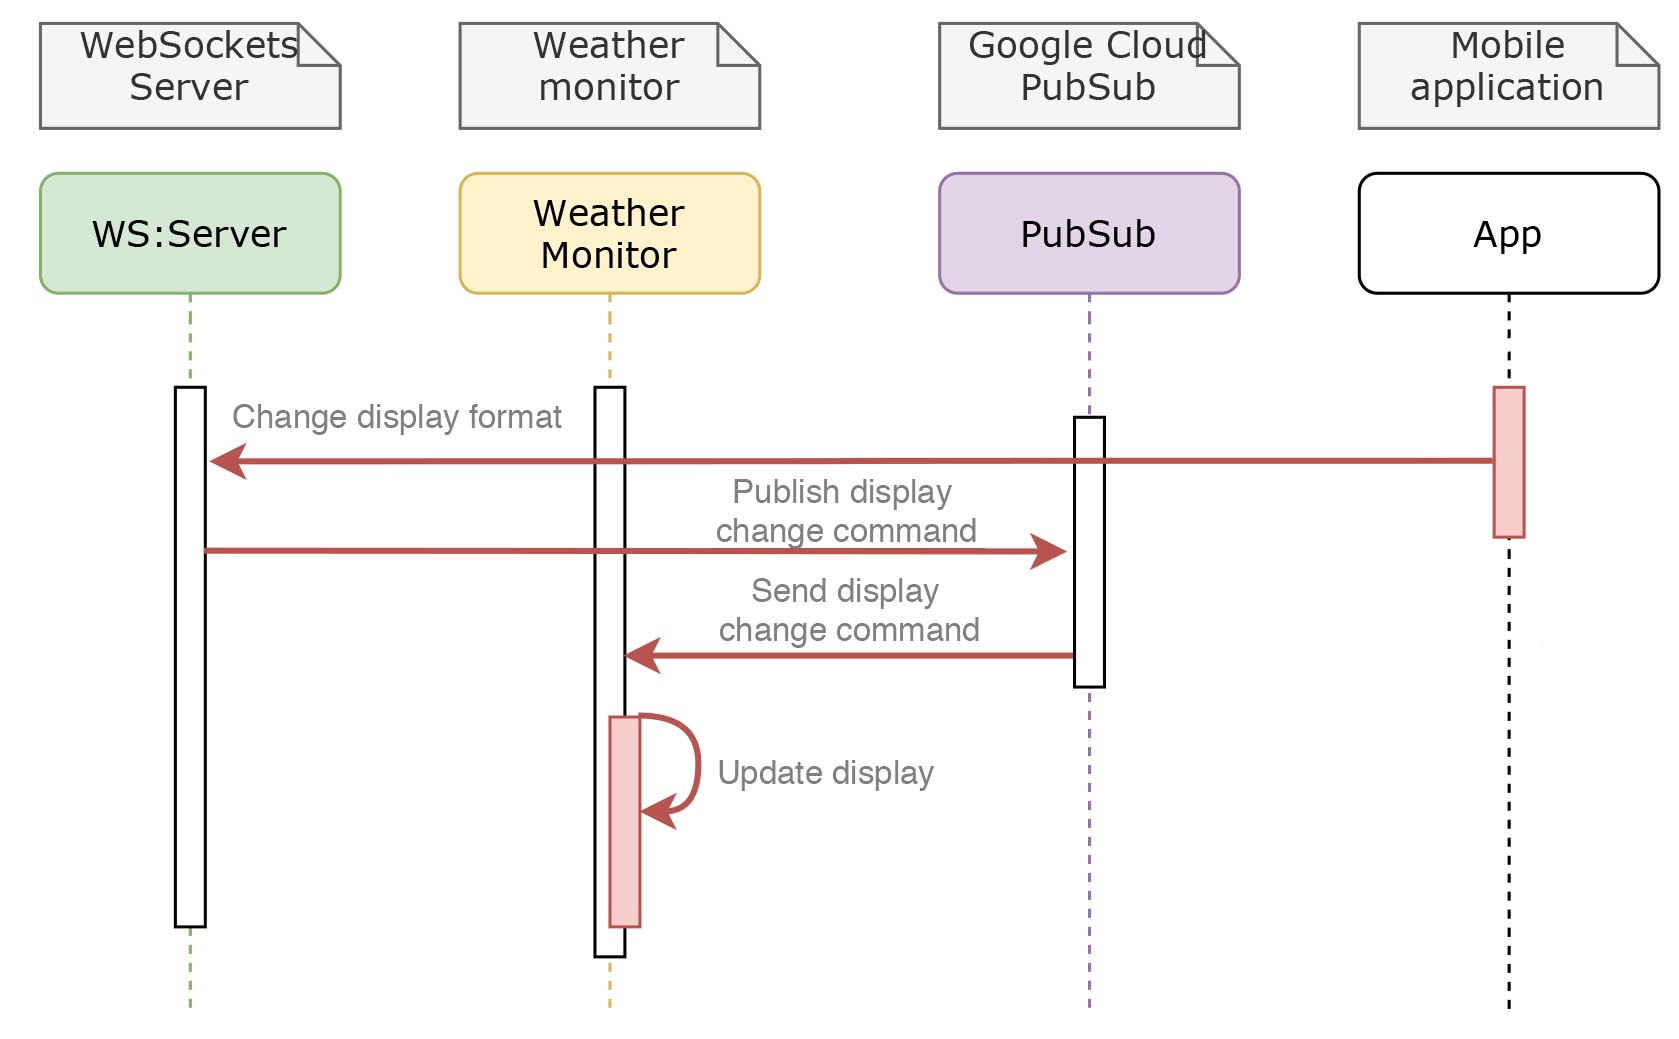
\includegraphics[width = 14cm]{figures/sub-diagram-2}
    \caption{Change displayed weather indicators - flow diagram}
    \label{fig:usecases}
\end{figure}

In Figure \ref{fig:faces_panel} one can see how will the weather monitor react the a display changes command. The visual feedback can vary in brightness - using the left side dial we can increase or decrease the brightness. 

\begin{figure}[!htb]
    \centering
    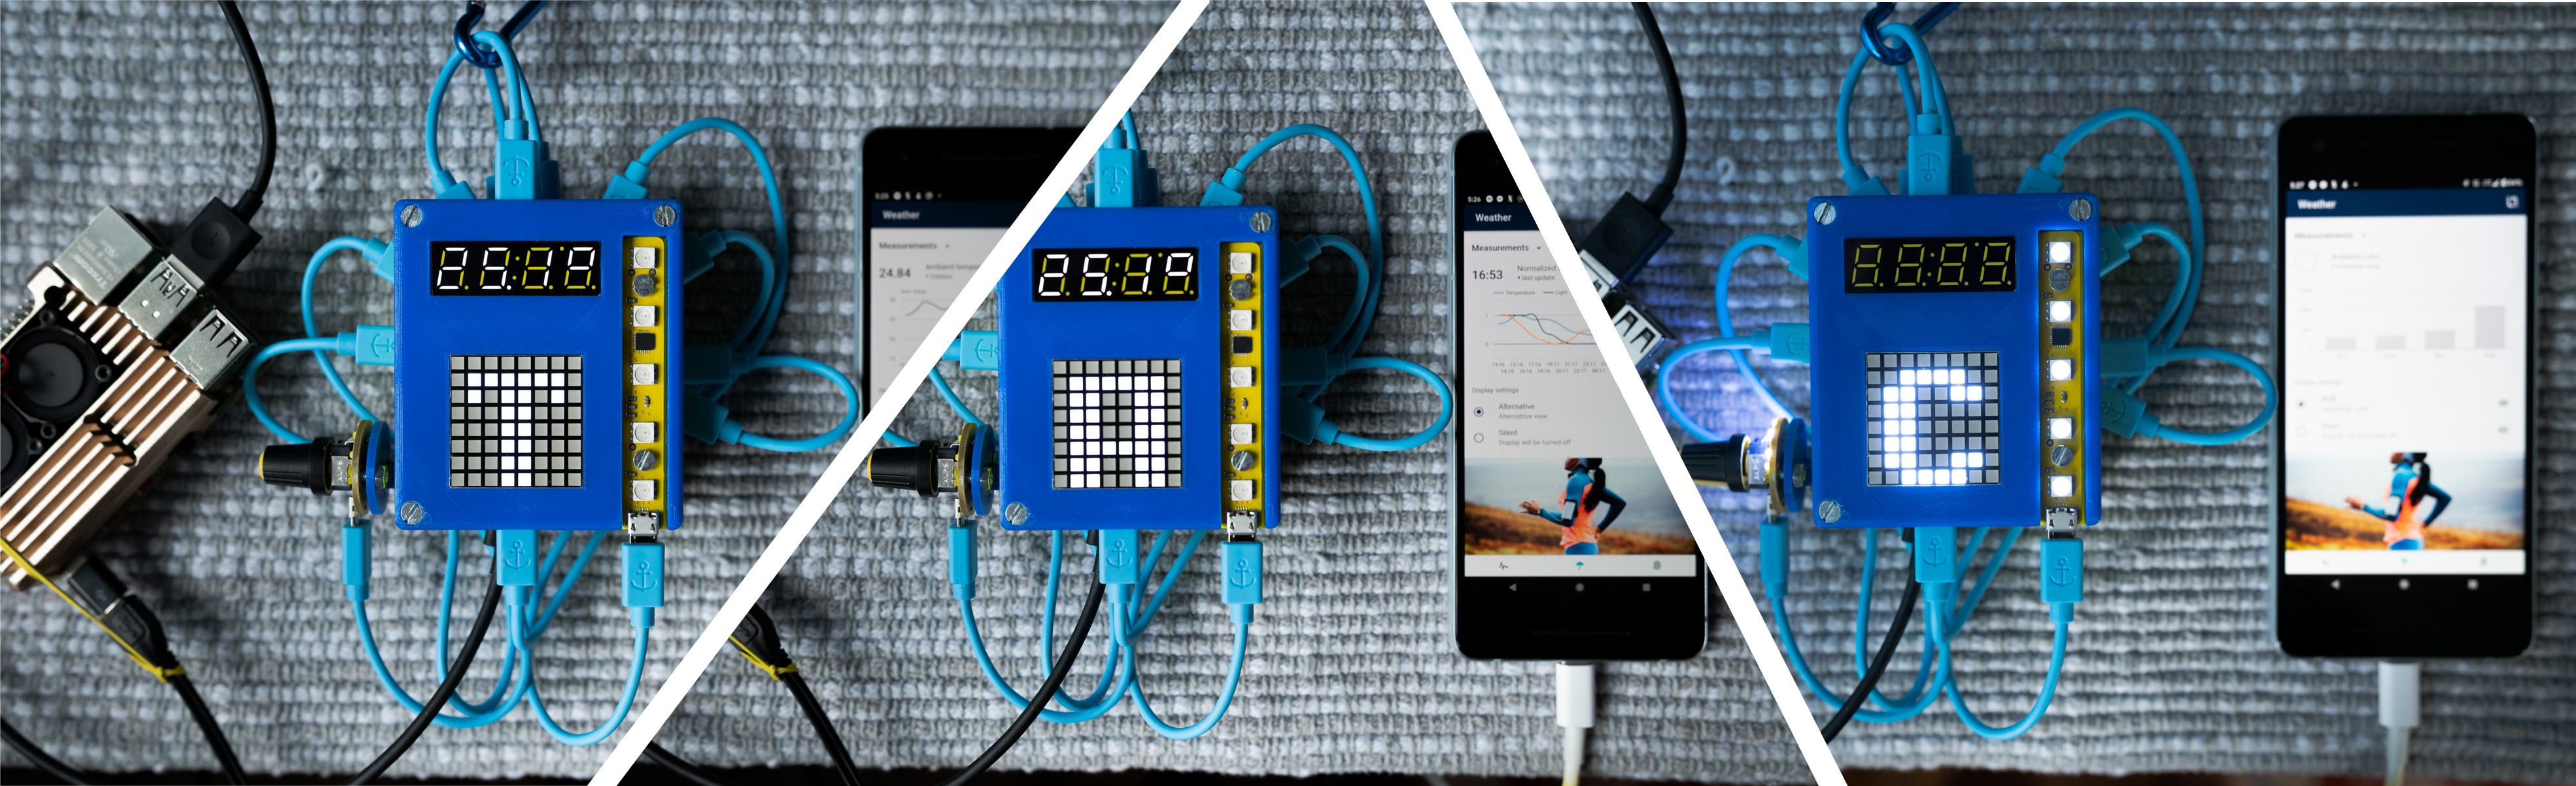
\includegraphics[width = 15.5cm]{figures/faces}
    \caption{Display options depicting Temperature, Alternative and Color modes}
    \label{fig:faces_panel}
\end{figure}

\vspace{4mm}
\textbf{3. Pair/Unpair a weather device}
\vspace{4mm}

There are a couple of reasons behind someone pairing or unpairing a weather device. One of them would be to pair a new device to the application, or stop the connection between devices as there is no reason to continue the communication.

\begin{table}[!htb]
  \begin{center}
    \label{tab:table90}
    {\begin{tabular}{p{5cm} p{12cm}}
        \textbf{Use case specifications} & \textbf{Description}\\
         Goal & \textbullet \hspace{1mm} begin or end the communication between the weather \\
         & device and the mobile application\vspace{2mm} \\
         Pre-condition & \textbullet \hspace{1mm} the weather station should be powered on and paired \\
          & or unpaired to the mobile app \\
          & \textbullet \hspace{1mm} the mobile device should have a consistent internet \\
          & connection\vspace{2mm}\\
         Post-condition & \textbullet \hspace{1mm} an user should see that the real-time data stopped \\ & updating, or it just started\vspace{2mm} \\
         Constraints / Issues / Risks & \textbullet \hspace{1mm} the weather station can enter an undefined state due \\ 
          & to a hardware issue\vspace{2mm} \\
                   Trigger Event(s) & \textbullet \hspace{1mm} - \\
         & - & 
         & - \vspace{2mm} \\
         Trigger Event(s) & \textbullet \hspace{1mm} a device can be paired by typing its serial number\\ 
         & in the "Pair (serial number)" input field found \\ 
         & in the "Monitor" $\rightarrow$ "Connected device" panel \\ 
         & \textbullet \hspace{1mm} to unpair a device, an user should tap on the green \\
         & cloud found on the right side of the "Currently \\
         & connected" list, found in the "Monitor" $\rightarrow$ \\
         & "Connected device" panel. \vspace{2mm} \\
         System Event(s) & \textbullet \hspace{1mm} a message is sent from the mobile app to the weather \\
         & device \vspace{2mm} \\
         Primary Actor & \textbullet \hspace{1mm} the user which owns the weather station\\
    \end{tabular}}
  \end{center}
\end{table}

In order to make it happen, a couple of endpoints exchange messages between them. In the following code snippets one can better understand the implementation behind this use case.

\begin{lstlisting}[language=Python, caption=IoT Data Sensing Layer: 1 (Light display execution sequence; runs until the thread is canceled)]
def pairing():
    subscriber = pubsub_v1.SubscriberClient()
    subscription_path = subscriber.subscription_path(
        'asavage2251', 'chappie-pairing')
    future = subscriber.subscribe(
        subscription_path, callback=pairing_callback)
    try: future.result()
    except Exception as exc:
        print('Pairing exception: ', exc); future.cancel()
\end{lstlisting}

\begin{lstlisting}[language=Python, caption=IoT Data Sensing Layer: 2 (Light display execution sequence; runs until the thread is canceled)]
def pairing_callback(message):
    data = message.data.decode('utf-8')
    try:
        message.ack()
        data = json.loads(data)
        if 'emit' in data:
            if data['emit']:
                display = True
                data_communication_thread = 
                    threading.Thread(target=data_communication)
                display_settings_thread = 
                    threading.Thread(target=display_settings)
                data_communication_thread.start()
                display_settings_thread.start()
            elif not data['emit']:
                display = False
                data_communication_thread.do_run = False
                display_settings_thread.do_run = False
    except Exception as exc:
        print('Pairing callback exception: ', exc)
\end{lstlisting}

\section{Implementation}

\subsection*{Software tools \& technologies}

Before reading about the architectural proposal, the software tools are really important to be stated, as one language can either support an architecture or raise a burden. One can identify the building blocks easier through code inspection, whilst others might find the visual identity of the tools we used more convenient in order to understand what technologies were involved. If neither, the system is based on four Google Cloud Services: PubSub, Dataflow, BigQuery and Monitor, while the weather station made used of a Raspberry Pi 4B computer, Pimoroni hardware and 3D printed parts obtained from a Prusa I3 MK3S. In terms of languages used, all servers and the Dataflow pipeline were written in Python3. The mobile application was built using the Ionic framework, implying that Typescript, HTML and CSS were also used.

\begin{figure}[!htb]
    \centering
    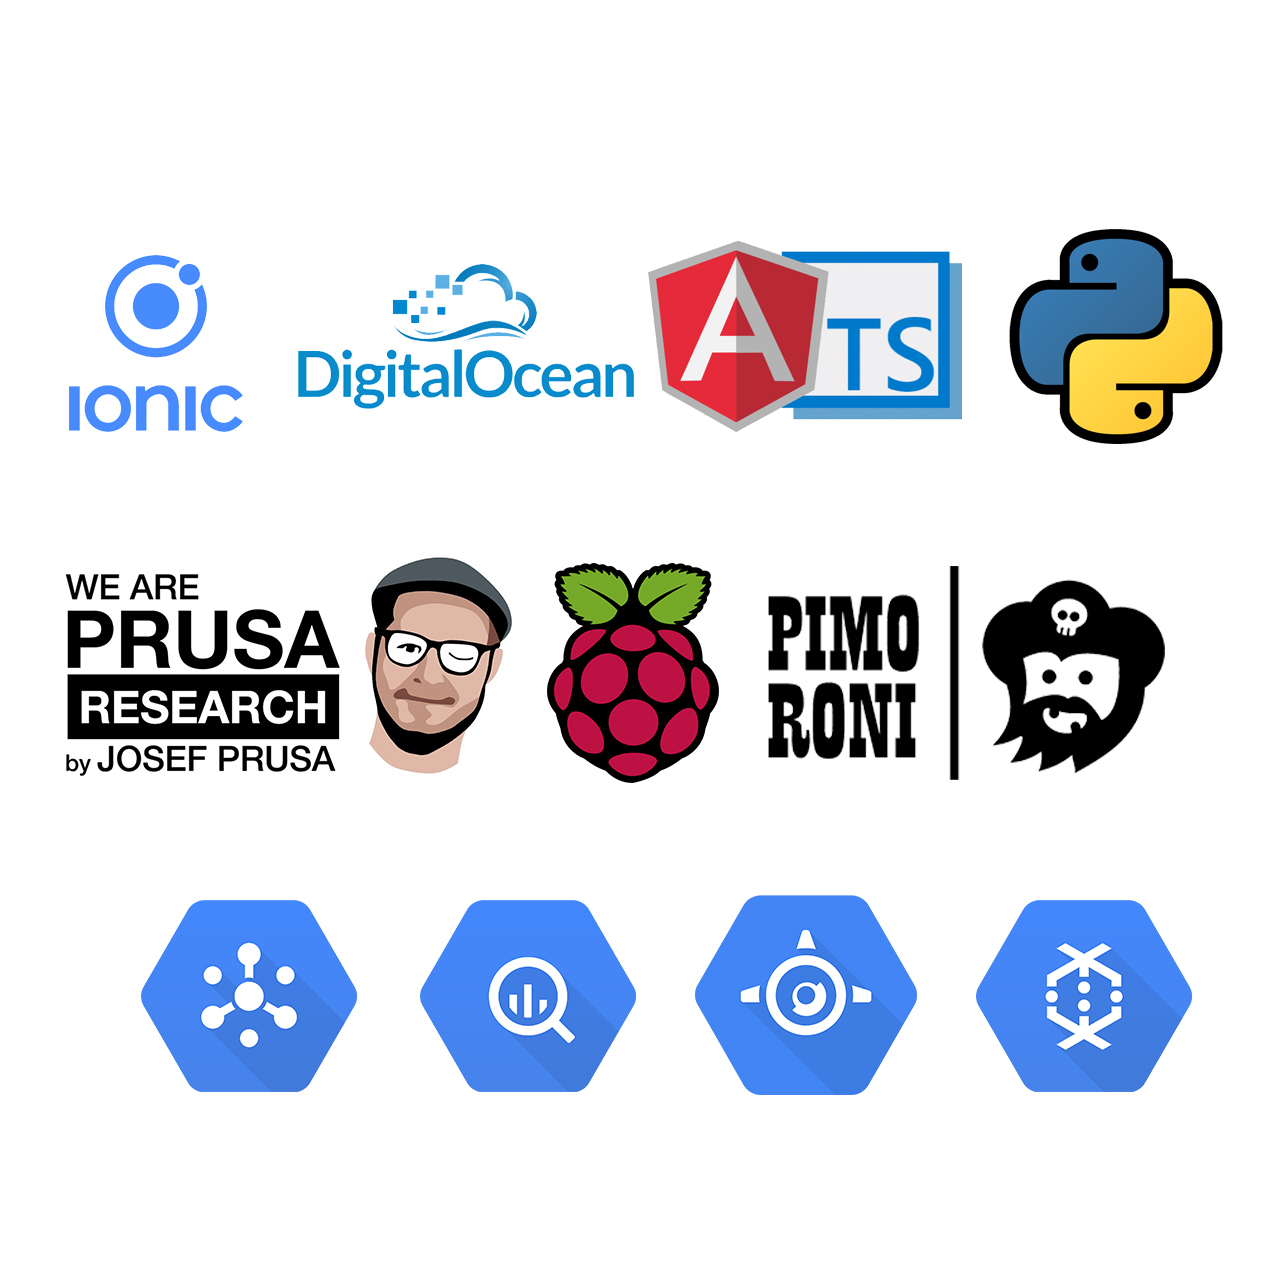
\includegraphics[width = 12cm]{figures/tools.jpg}
    \caption{Software tools, languages and frameworks used}
    \label{fig:app_flow}
\end{figure}

\subsection*{Development}

Google's first release of a Python SDK for Cloud Dataflow goes back as far as the 27th of July, 2016, yet it was not a tool ready for development at that time. Besides offering an SDK, Google is building part of their tools in \textbf{Python}, so are Netflix, Spotify and Dropbox. Why are these companies important to the discussion we have in this paper? They are among many other companies that are constantly evolving, building products compatible with major platforms and systems. Python simplifies complex software development, offering many open source frameworks and tools, with a robust standard library. Dropbox used  According to \cite{pypl}, Python had a growth of popularity that placed it on the first place for the year 2020.

\begin{figure}[!htb]
    \centering
    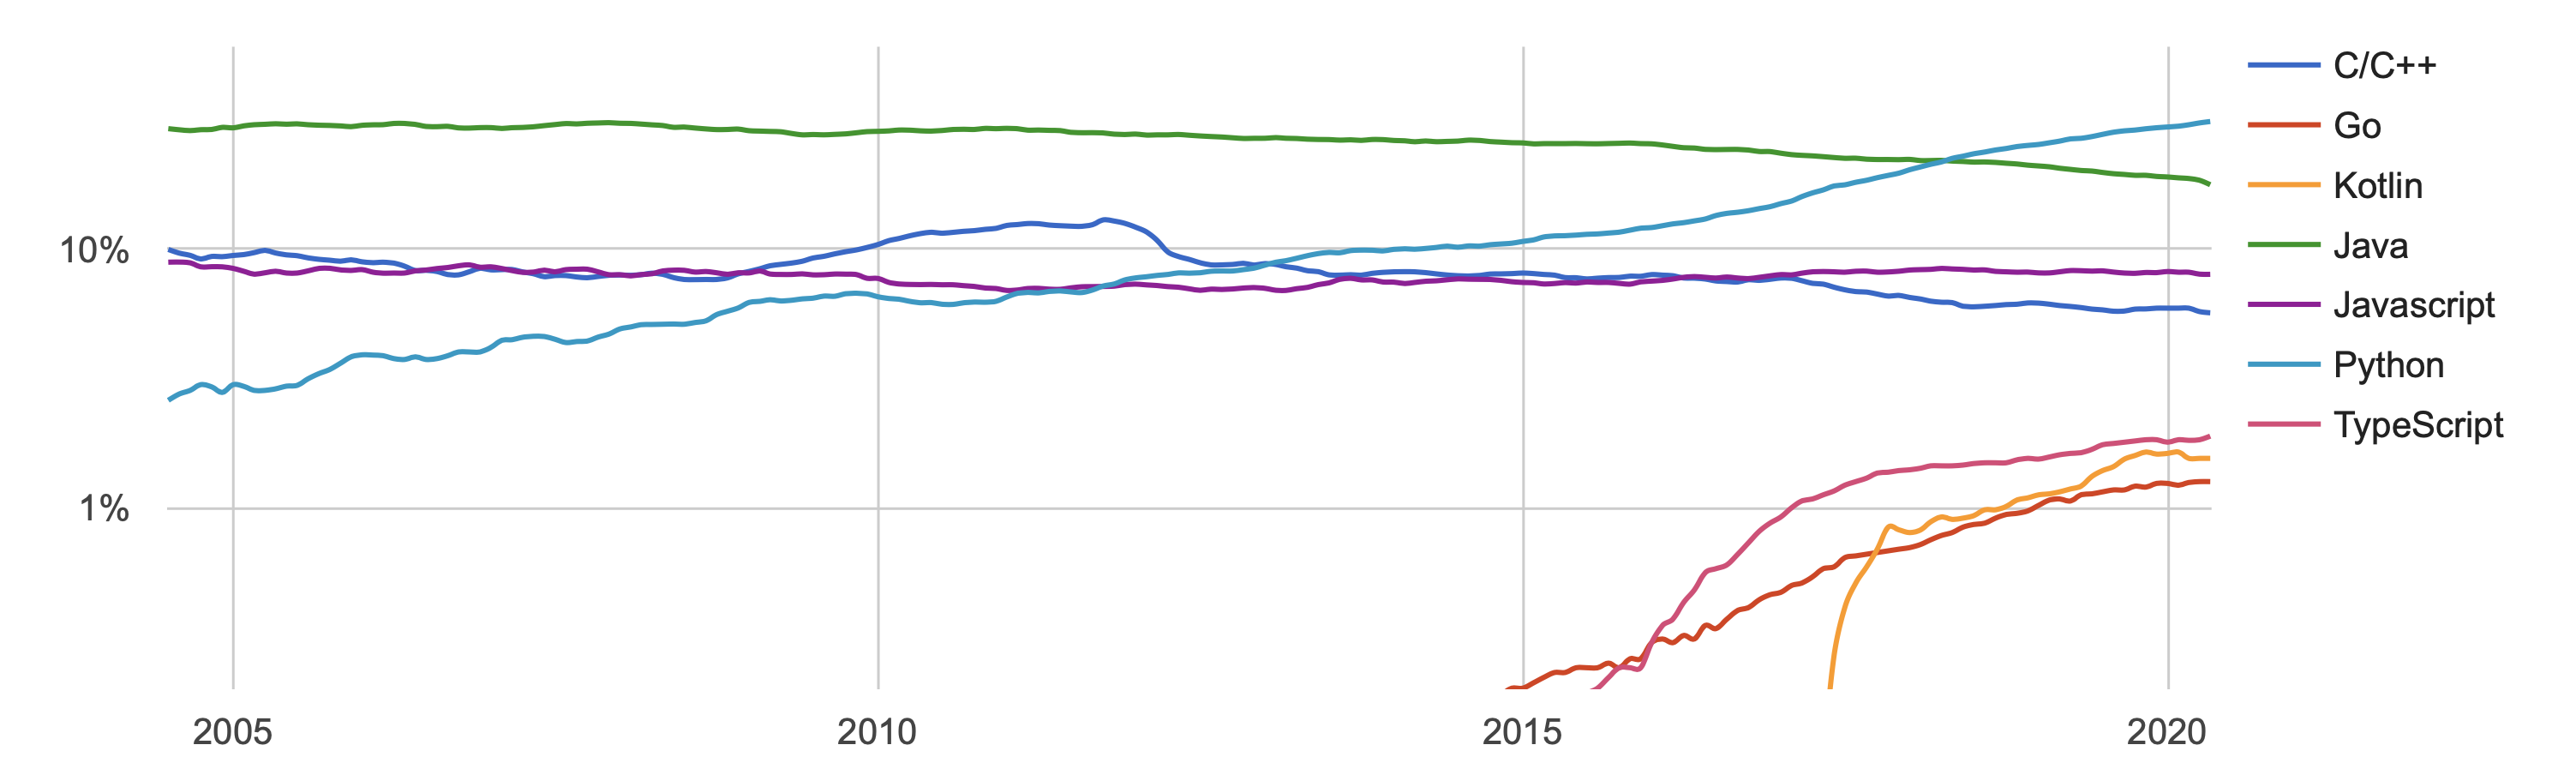
\includegraphics[width = 15.5cm]{figures/python_pop}
    \caption{2020 programming languages popularity comparison \cite{pypl}}
    \label{fig:f1}
\end{figure}

However common, the \textbf{visualization tools} had to simultaneously display data sets on a broad range of values. For example, how do we represent a temperature value with a lower bound of -50 and a upper bound of 50 on the same chart with an air pressure value that is usually stationary at over 9000. One answer is to \textbf{normalize the values} as depicted in the formula below, where v is the row value, nv is the normalized value, lower case m stands for the minimum value ever recorded for that measurement type, while capital case M represents the maximum.

\begin{equation}
nv_i = \frac{v_i - m_i}{M_i - m_i}  
\end{equation}

The \textbf{data flow} that takes place on the cloud is described by the content of the file `chappie-pipeline.py`. In order to ease the development workflow, it would be useful to create a virtual environment so that the libraries will remain available for next time when we are accessing the machine. At the moment when this project was built, one requirement that might not seem obvious, yet it is required is the `google-api-python-client`, which has to be installed. Changes can be made to the source file by simply switching between bash and finder panels in the GCP console. If successful, the prompt should display:
\begin{lstlisting}[language=bash]
JOB_MESSAGE_DETAILED: Workers have started successfully.
\end{lstlisting}

\clearpage
\subsection{Challenges encountered}

This section does not approach a different discussion, but it is presenting the implementation challenges - those points where something notable happened, and we found them interesting enough to share with the reader.

\subsubsection{Operating system setup}

When we bought the first set of sensors from Pimoroni we had some issues as their library was no longer maintained, or it was not a priority for those involved at the moment. After a search, there were very few solutions, but even so, one seemed promising. After a few hours, we managed to solve the errors we had and also posted on Stackoverflow. 

\begin{figure}[!htb]
    \centering
    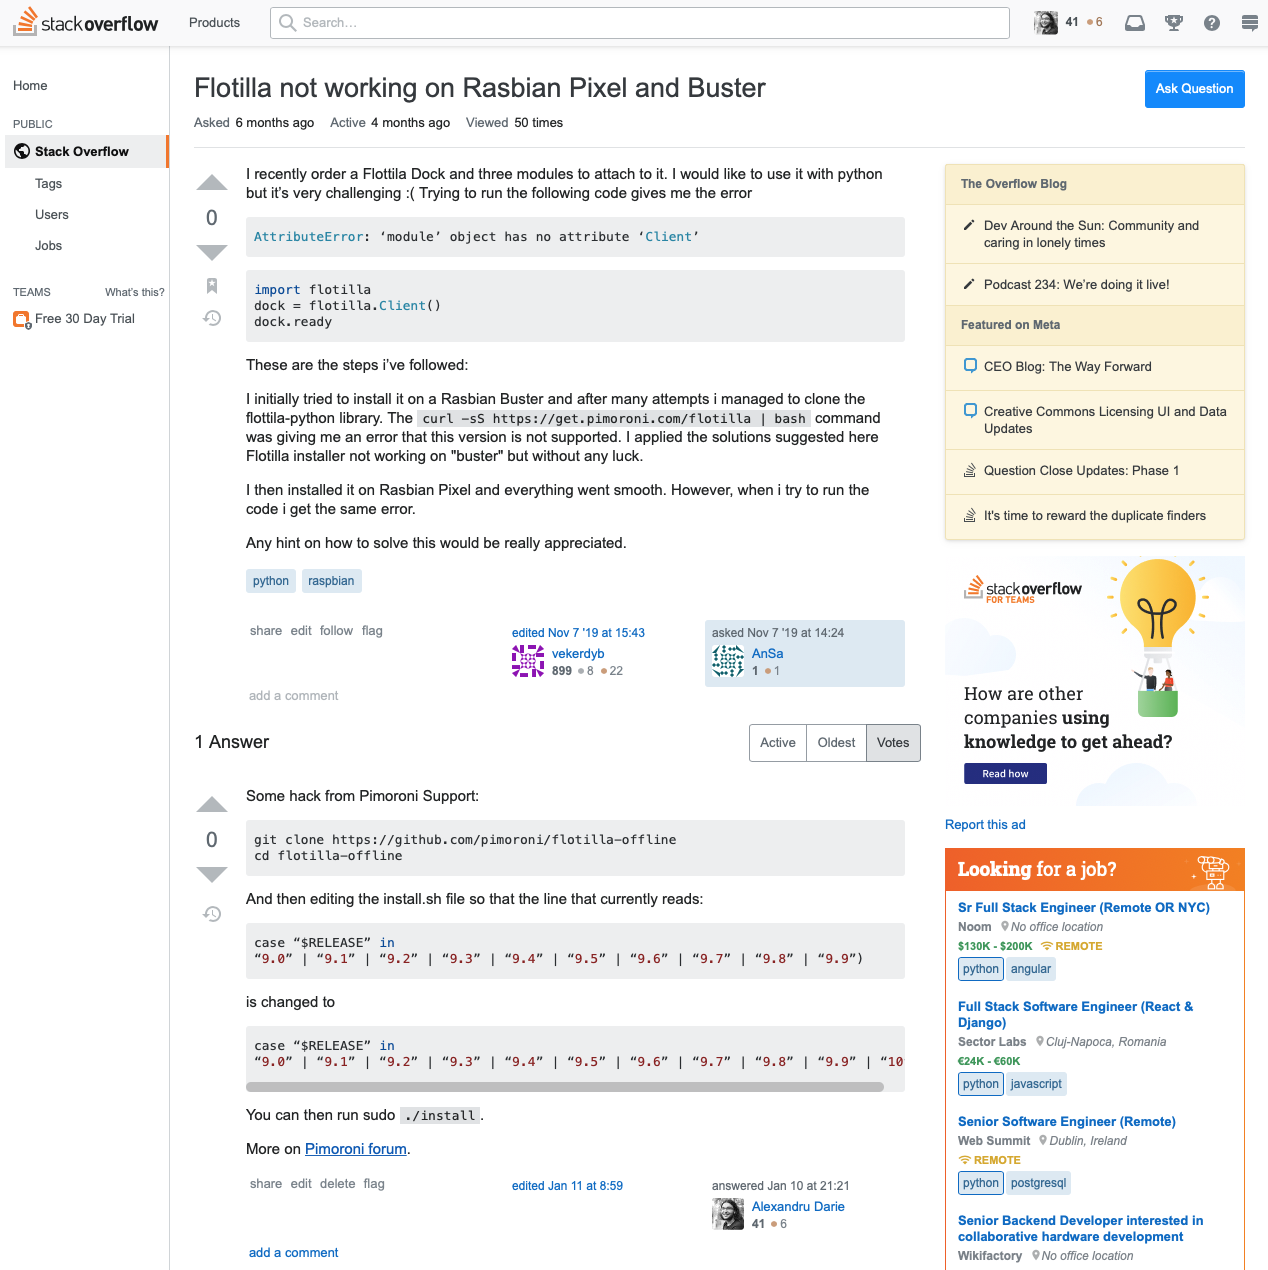
\includegraphics[width = 15.5cm]{figures/sde2}
    \label{fig:sde2}
\end{figure}

After successfully installing the operating system using the balenaEtcher tool, a few modifications were made to the standard library distribution offered by Pimoroni for the Flotilla suite of sensors. The solution \cite{stovlf} was made publicly available on www.stackoverflow.com as a response to an existing question.

\begin{lstlisting}[language=bash]
user$ git clone https://github.com/pimoroni/flotilla-offline
user$ cd flotilla-offline
\end{lstlisting}

\hspace{-6mm}And then editing the install.sh file so that the line that currently reads

\begin{lstlisting}[language=bash]
case "$RELEASE" in
"9.0" | "9.1" | "9.2" | "9.3" | "9.4" | "9.5" | "9.6" | "9.7" | "9.8" | "9.9")
\end{lstlisting}

\hspace{-6mm}is changed to

\begin{lstlisting}[language=bash]
case "$RELEASE" in
"9.0" | "9.1" | "9.2" | "9.3" | "9.4" | "9.5" | "9.6" | "9.7" | "9.8" | "9.9" | "10")
\end{lstlisting}

\hspace{-6mm}We can then run 

\begin{lstlisting}[language=bash]
user$ sudo ./install
user$ curl -sS https://get.pimoroni.com/flotilla | bash
\end{lstlisting}

\hspace{-6mm} Later, we wrote an email to one of Pimoroni's developers and it got patched.

\subsubsection{Front-end message ingestion using the producer-consumer pattern}

In order to deliver the real-time aspect of the entire application we used a producer-consumer layer built on web sockets \cite{ws}. The intuitive approach of searching a front-end package to consume data does not apply in a context of no REST API, therefore:
\begin{table}[!htb]
  \begin{center}
    \label{tab:table10}
    \resizebox{\textwidth}{!}{\begin{tabular}{l|l|l}
      \textbf{Component description} & \textbf{Undertaken action} & \textbf{Machine}\\
      the mobile app became a consumer & listen host:port & \\
      \hline
      a server & traffic distribution between the producer and the consumer & host:port \\
      \hline
      the PubSub subscriber became a producer & send host:port & \\
    \end{tabular}}
  \end{center}
\end{table}

\subsection{Limitations}

Any hardware has its limitations. Below we'll discuss about them. Raspberry Pi \& Flotilla sensors - sensors error and specifications. Must read the tech sheets and make a table with their errors and other specifications.

\begin{table}[!htb]
  \begin{center}
    \label{tab:table4}
    \caption{Hardware specifications: Pimoroni's Flotilla series}
    \resizebox{\textwidth}{!}{\begin{tabular}{l|l|l|l}
      \textbf{Purpose} & \textbf{Device name} & \textbf{Description} & \textbf{Notes}\\
      \hline
        Connection & Dock & It talks, through serial USB, to all of the Flotilla & Use up to four docks at once \\
        & & modules connected to its eight ports & ATMEGA32A4U microcontroller \\
      \hline
        Sensors & Weather & Reads temperature and pressure & BMP280 sensor \\
        & Light & Detects ambient light level & TSL2581 sensor \\
      \hline
        Display & Matrix & An 8x8 white LED matrix & White LED \\
        & Rainbow & The module has five shiny bright full-colour LEDs & Five 5050 RGB LEDs\\
    \end{tabular}}
  \end{center}
\end{table}

The software has its own limitations, being one of the reasons for having a future work section, but not only. Strava API represents a valuable source of information, yet it left room for improvements, with documentation that lacks in certain aspects and endpoints that could have offered better structured information. Nevertheless, these observations were made from our standpoint, and they concern our interests. Google Fit will be analyzed in a following version of this paper as a potential fitness activity source point.

\section{Results}

With no reason for a thoroughly investigation of the machine learning techniques, we felt the responsibility of giving some explanations with regard to the results we obtained.

\subsection*{Discussions and comparison}

The main interest of this application is to find the ideal weather for certain types of outdoor activities, defined as the temperature, ambient light, and air pressure triplet. Because the values of any of the three measurements are continuous and have a constant slope, this problem can be approached with the linear regression method. This supervised machine learning approach is directly accessible from the Google Cloud BigQuery service, eliminating the need for moving data between nodes in a distributed system. Analyzing data and retraining models in a production environment using SQL queries brings value to the final product and allows for more granular control over the model options and the rows used for training.

\begin{lstlisting}[language=SQL]
CREATE or REPLACE MODEL models.temperature_prediction
OPTIONS(
 model_type='linear_reg', 
 labels=['avg_temperature'], 
 max_iterations=20) AS 
WITH  
 params AS (SELECT 1 AS TRAIN, 0 AS EVAL),
 habits AS (
    SELECT avg_temperature, avg_air_pressure, 
    EXTRACT(HOUR FROM start_date
 ) AS hourofday,
 FROM `habits`, params
 WHERE type = "Run" and distance > 0 and moving_time > 0 and avg_temperature IS NOT NULL and MOD(ABS(FARM_FINGERPRINT(CAST(start_date AS STRING))), 2) = params.TRAIN and TIMESTAMP_DIFF(CURRENT_TIMESTAMP(), start_date, DAY) <= 30)
SELECT * FROM habits;
\end{lstlisting}

One query may take into consideration the running habits stored over the last 30 days in a training session. If no column was named \textit{label}, then \textit{input\_label\_cols} must contain the column value we want to predict. \cite{a2} The best model was obtained using as input values the air pressure and the outdoor activity starting hour in the prediction of temperature, with an MAE of 1.45516, an RMSE of 1.76486, and a normalized RMSE of 0.18445. A Root Mean Square Error of ~1.76 can be evaluated as ±1.76 °C, so instead of predicting an actual value of 23 °C, the model might return 24.76 °C or 21.24 °C. In terms of thermal thresholds, "a person can be unaware of a 4-5 °C change in temperature, provided that the temperature of the skin remains within the neutral thermal region of 30-36 °C". \cite{a1} Other input values gave models with predictions in the same range of 4-5 °C off.

\begin{figure}[!htb]
    \centering
    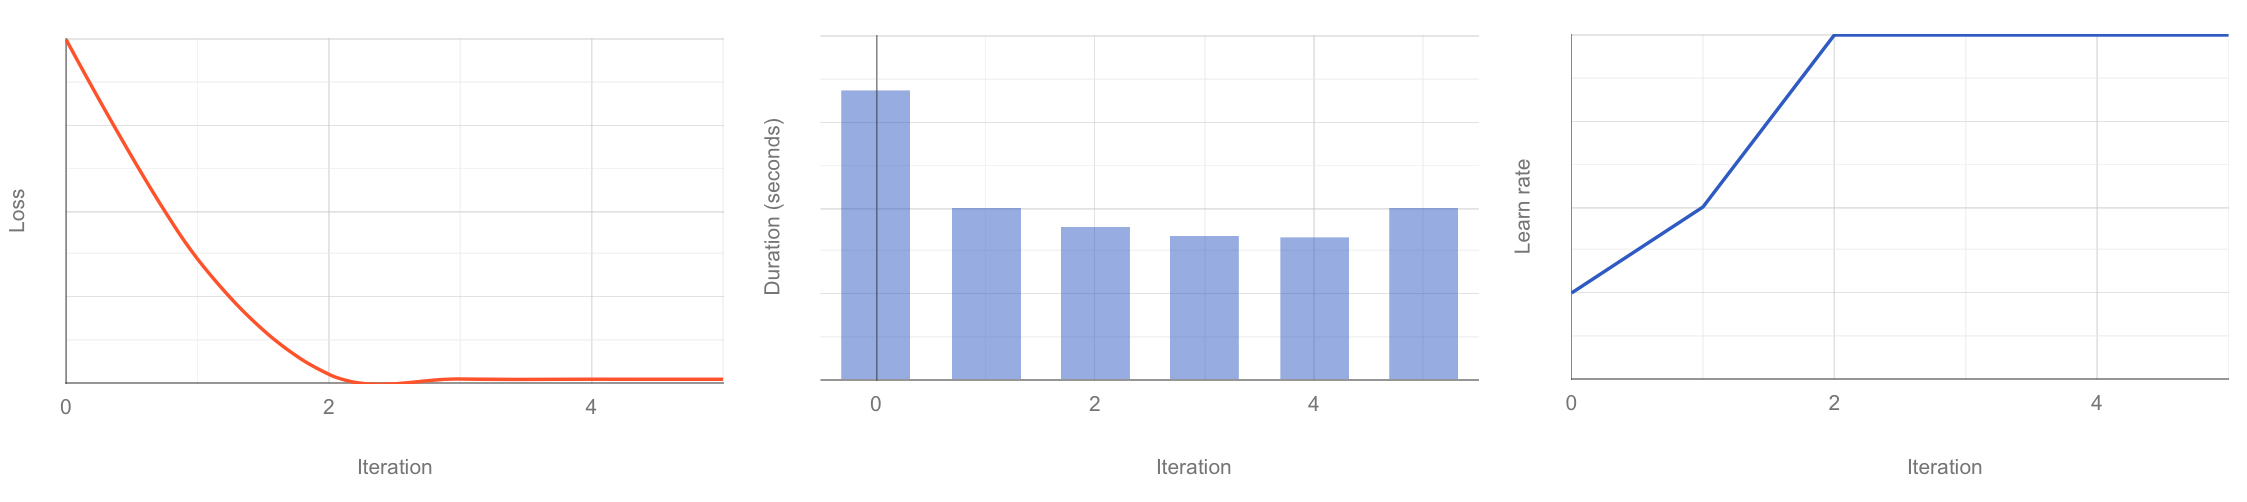
\includegraphics[width = 15.5cm]{figures/lr.jpg}
    \caption{Linear regression training execution details}
    \label{fig:app_flow}
\end{figure}

Due to the small carnality of such data input, namely the number of outdoor activities a person can participate in during a month, the BigQuery ML trains the model faster by computing a closed-form solution. \cite{a3} Google's infrastructure can produce a difference in term of time spent on training, yet only for a subset of machine learning problems with either a small number of features, more rows than features, or doing linear regression without L1 regularization, there is a faster algorithm that finds a closed-form solution by computing the Moore-Penrose pseudo-inverse.

\subsection*{Accuracy}

To the best of our knowledge, there are no datasets, neither results for this specific problem, so that we can only follow some statistical methods to document the accuracy. 

\begin{table*}[!htb]
    \centering
    \begin{threeparttable}
    \begin{tabular}{|l|*{5}{c|}}\hline
        \backslashbox[3.75cm]{Features\tnote{1}}{Metric}
        &\makebox[4em]{MAE}&\makebox[4em]{RMSE}&\makebox[4em]{NRMSE}\\\hline\hline
        avg\_temperature & 1.455167 & 1.764866 & 0.184458\\
        avg\_light & & & \\
        avg\_air\_pressure & & & \\
        \hline
        avg\_temperature & 1.455392 & 1.766873 & 0.184877\\
        avg\_light & & & \\
        avg\_air\_pressure & & & \\
        hour\_of\_day & & & \\
        \hline
        avg\_temperature & 1.466996 & 1.769391 & 0.185405\\
        avg\_air\_pressure & & & \\
        hour\_of\_day & & & \\
        \hline
        avg\_temperature & 1.576829 & 1.845601 & 0.201720\\
        hour\_of\_day & & & \\
        \hline
        avg\_temperature & 1.743081 & 2.009224 & 0.239073\\
        distance & & & \\
        elapsed\_time & & & \\
        average\_speed & & & \\
        \hline
        avg\_temperature & 2.118429 & 2.711958 & 0.435552\\
        avg\_light & & & \\
        avg\_air\_pressure & & & \\
        distance & & & \\
        elapsed\_time & & & \\
        hour\_of\_day & & & \\
        \hline
        
    \end{tabular}
    \begin{tablenotes}
      \small
      \item[1] Each row describes the set of features selected for training, and the experimental results obtained.
    \end{tablenotes}
\caption{Feature selection comparison}
\label{results}
\end{threeparttable}
\end{table*}

To improve the model, once we evaluated the performance of the initial model, we can go back and forth, pruning or attaching new features to the old ones, so that we can get a better model. The following table depicts some of the training sessions made using the above query structure on a data set of 90 entries, with an average temperature of 16.885964. This temperature value was used in the Normalized Root Mean Squared Error formula:

\begin{equation}
NRMSE = \frac{\sqrt{\frac{1}{n} * \sum_{i=1}^{n} (p_i - a_i)^2}}{\overline{v}}  
\end{equation}

The best model described in this the Table \ref{results} is also the one used in the project implementation. Feature selection..

\section{Testing \& monitoring}

\subsection*{Means of testing}

"Software testing is a sport like hunting, it's bughunting." - Amit Kalantri.

From concept to production we encounter three stages: build, review and refine. Testing the system, from a software engineering point of view, involved validation and verification, system, integration and unit testing, but due to the system specifications, they were mainly manually tested. 
The testing levels used in the development of the app were unit testing through adequate frameworks (pytest more explicitly) and integration and system testing by means of manual testing (with more emphasis on the last two). Due to the reliance on external services like Strava API and DigitalOcean, only small components independent of them could be unit tested, like the auxiliary functions in the Backend Server. The strategy adopted in the implementation of these tests was the black-box method since it enabled the developer to detach themselves from the written code and have a more critical look at the behaviour of the functions for boundary values. In the case of the integration testing, the methodology used was bottom-up. Firstly, we gradually tested the functionalities of the Backend Server until it was ensured that it works properly (in this case, the integration was explicitly with the Strava API and the database). Then, the mobile application functionalities which were independent of the Backend Server were guaranteed to work (namely the ones which interact directly with the Strava API). The system testing (which can also be seen as the final step of the integration testing) finally occurred when the features of the mobile dependent on the Backend Server needed to be verified that work. The choice of manual testing in the case of these levels was made because of the scale of the application which, from the developer's point of view, was a small one.

\subsection*{Monitoring}

Due to its design, this application was difficult to test and required a lot of time, as the problems that occurred had to be searched on four different machines. Each part was manually tested after it has been previously unit-tested. Google Cloud Platform offered a lot of tools for a consistent and bug-free development. Throughout the project, we used the Monitoring panel to observe the behavior of the system over time interval ranging from 7 days, up to 1 month.

\begin{figure}[!htb]
    \centering
    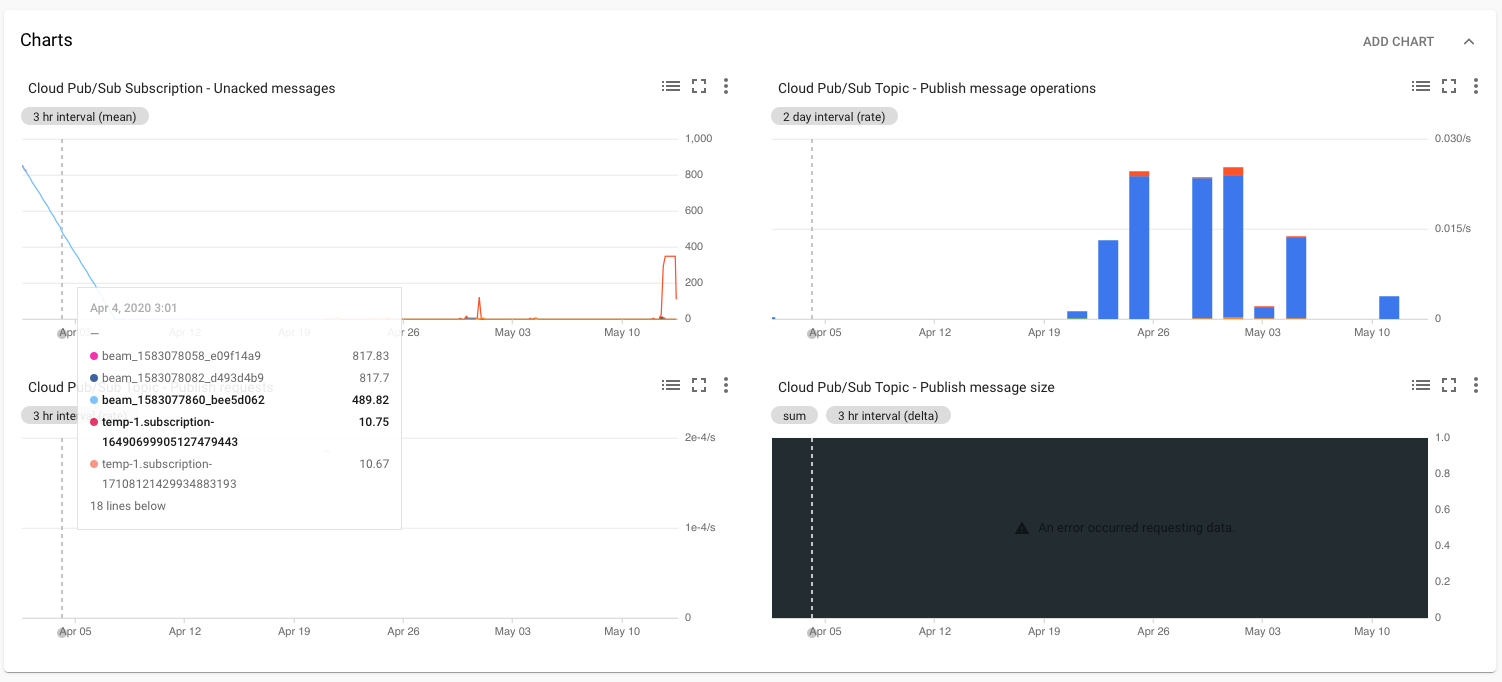
\includegraphics[width = 15.5cm]{figures/testing1}
    \caption{Monitoring the application using the Cloud console panels}
    \label{fig:f1}
\end{figure}

\clearpage
\section{Use manual}

Arguably as important as the ease with which we use the mobile application is also the simplicity of building the weather station. One can build it with as much as a screw driver, in less than 10 minutes. Nevertheless, the model depicted in Figure \ref{fig:weather_station_pres} is one of many models that have been manufactured for this project, over the last months. In the image are depicted the chassis components, the three sensors, a yellow dial module, the number and matrix display components, the Flotilla dock and a set of cables used to connect them.

\begin{figure}[!htb]
    \centering
    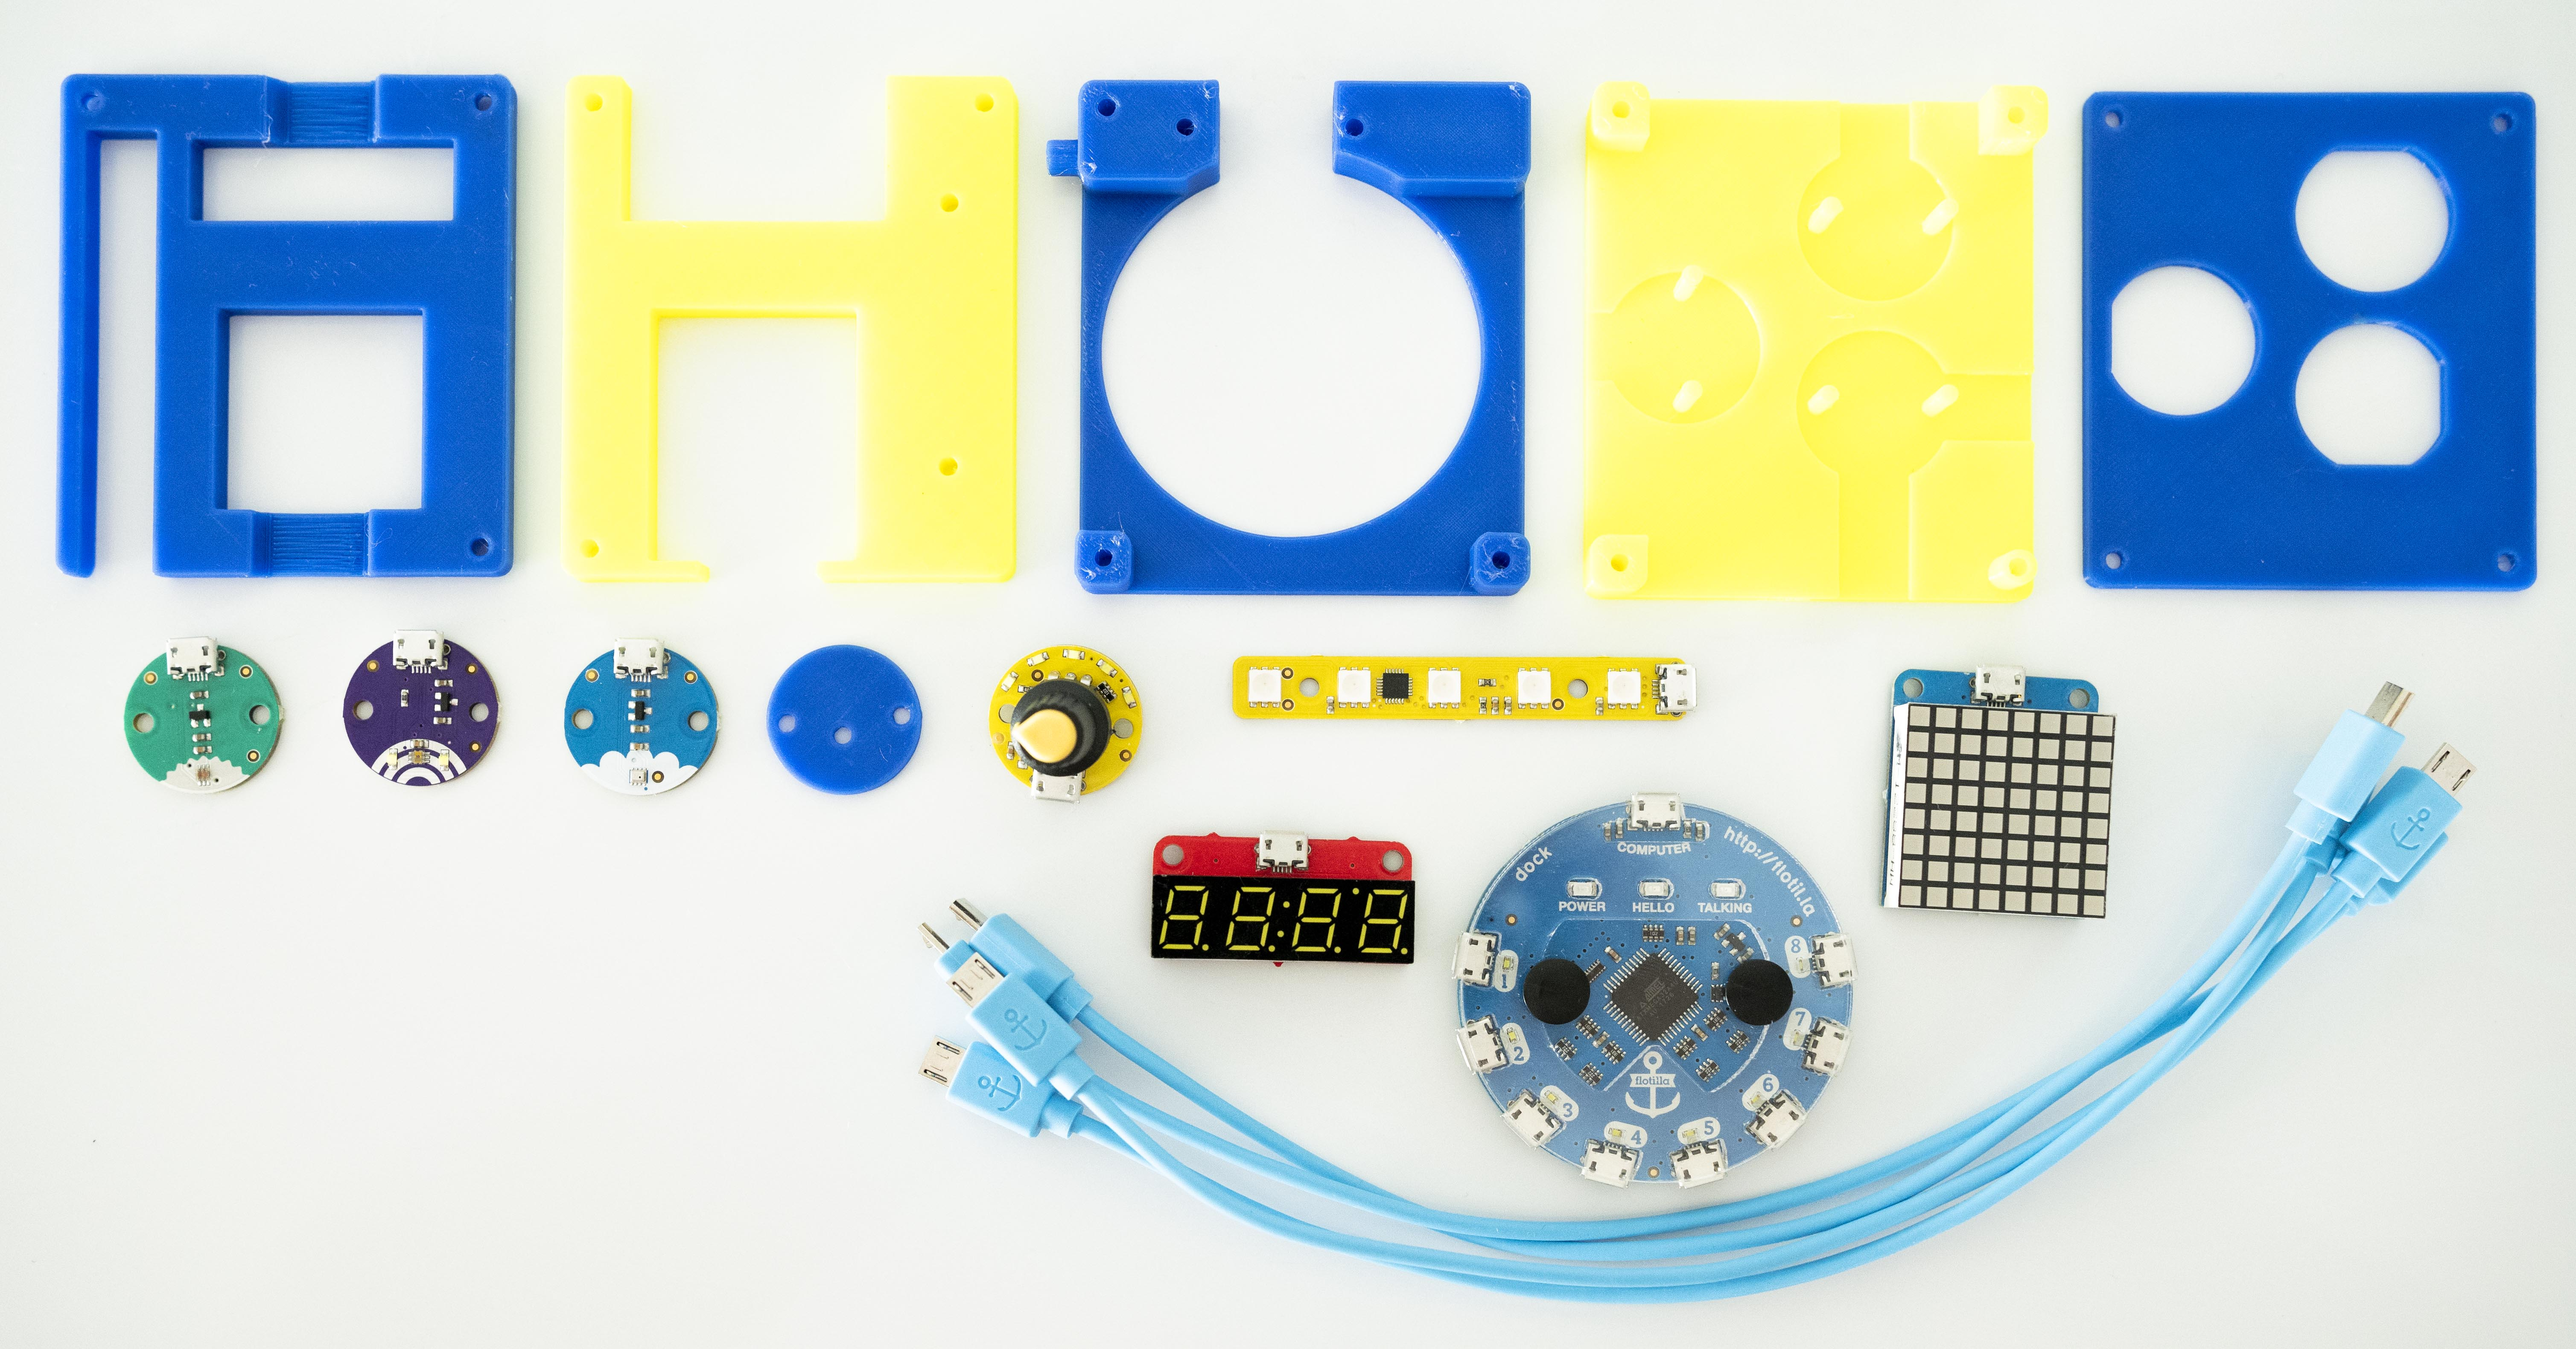
\includegraphics[width = 15.5cm]{bachelor/figures/FRO_3138}
    \caption{Weather station assembly overview}
    \label{fig:weather_station_pres}
\end{figure}

In Figure \ref{fig:assembly_line} is depicted visual representation of the manufacturing process, which was, of course, simplified so that it can be captured in a series of pictures. The main body is defined by a 70mm x 80mm x 34.5mm chassis of PLA, or polylactide - a thermoplastic polyester with a melting point of 150 to 160 °C. More on its limitations was described in the section 3.3.1.

\begin{figure}[!htb]
    \centering
    \includegraphics[width = 15.5cm]{bachelor/figures/assembly}
    \caption{Weather station assembly process}
    \label{fig:assembly_line}
\end{figure}

The main objective of this application is to enable people discover fitness habits in regards to the weather conditions. Mainly, it has three tabs, each of them describing one key feature: habits, weather monitor and athlete's fitness profile. Each of these tabs have an additional panel from which one can call for a particular sub-action. 

\subsection{Fitness habits}

Centering the whole weight of this project on one particular features makes it incredibly difficult to describe and develop, yet someones habits are no miracle and they can be known by someone without using a mobile application. Nevertheless, the reason behind building it is to help athletes that are not aware of their behaviour. Those being said, in the fitness habits panel we start from a comparison chart, which visually describes the differences between the current weather status and someones habits. If a potential user has any doubts, under the chart are listed the most recent five or less activities, depending on the activity type. Furthermore, if the decision should imply data reasoning, then one can take a decision based on its preferences numerically depicted in the left upper side of the first slide, the number of km predicted for a certain hour of the day, its probability to engage in any fitness activity for that day, or the overall statistics for the given season. The final slide of the habits panel describes data recorded up to 2 years ago, also stating the error in prediction in a human readable format. It was meant to give information on the model accuracy over time. In order to trust a tool, it has to be clear how far it can go at any point in time. Knowing the prediction error is not something that only the developers should know, as someone's health might be influenced by these predictions.
\vspace{4mm}

\begin{figure}[!htb]
    \centering
    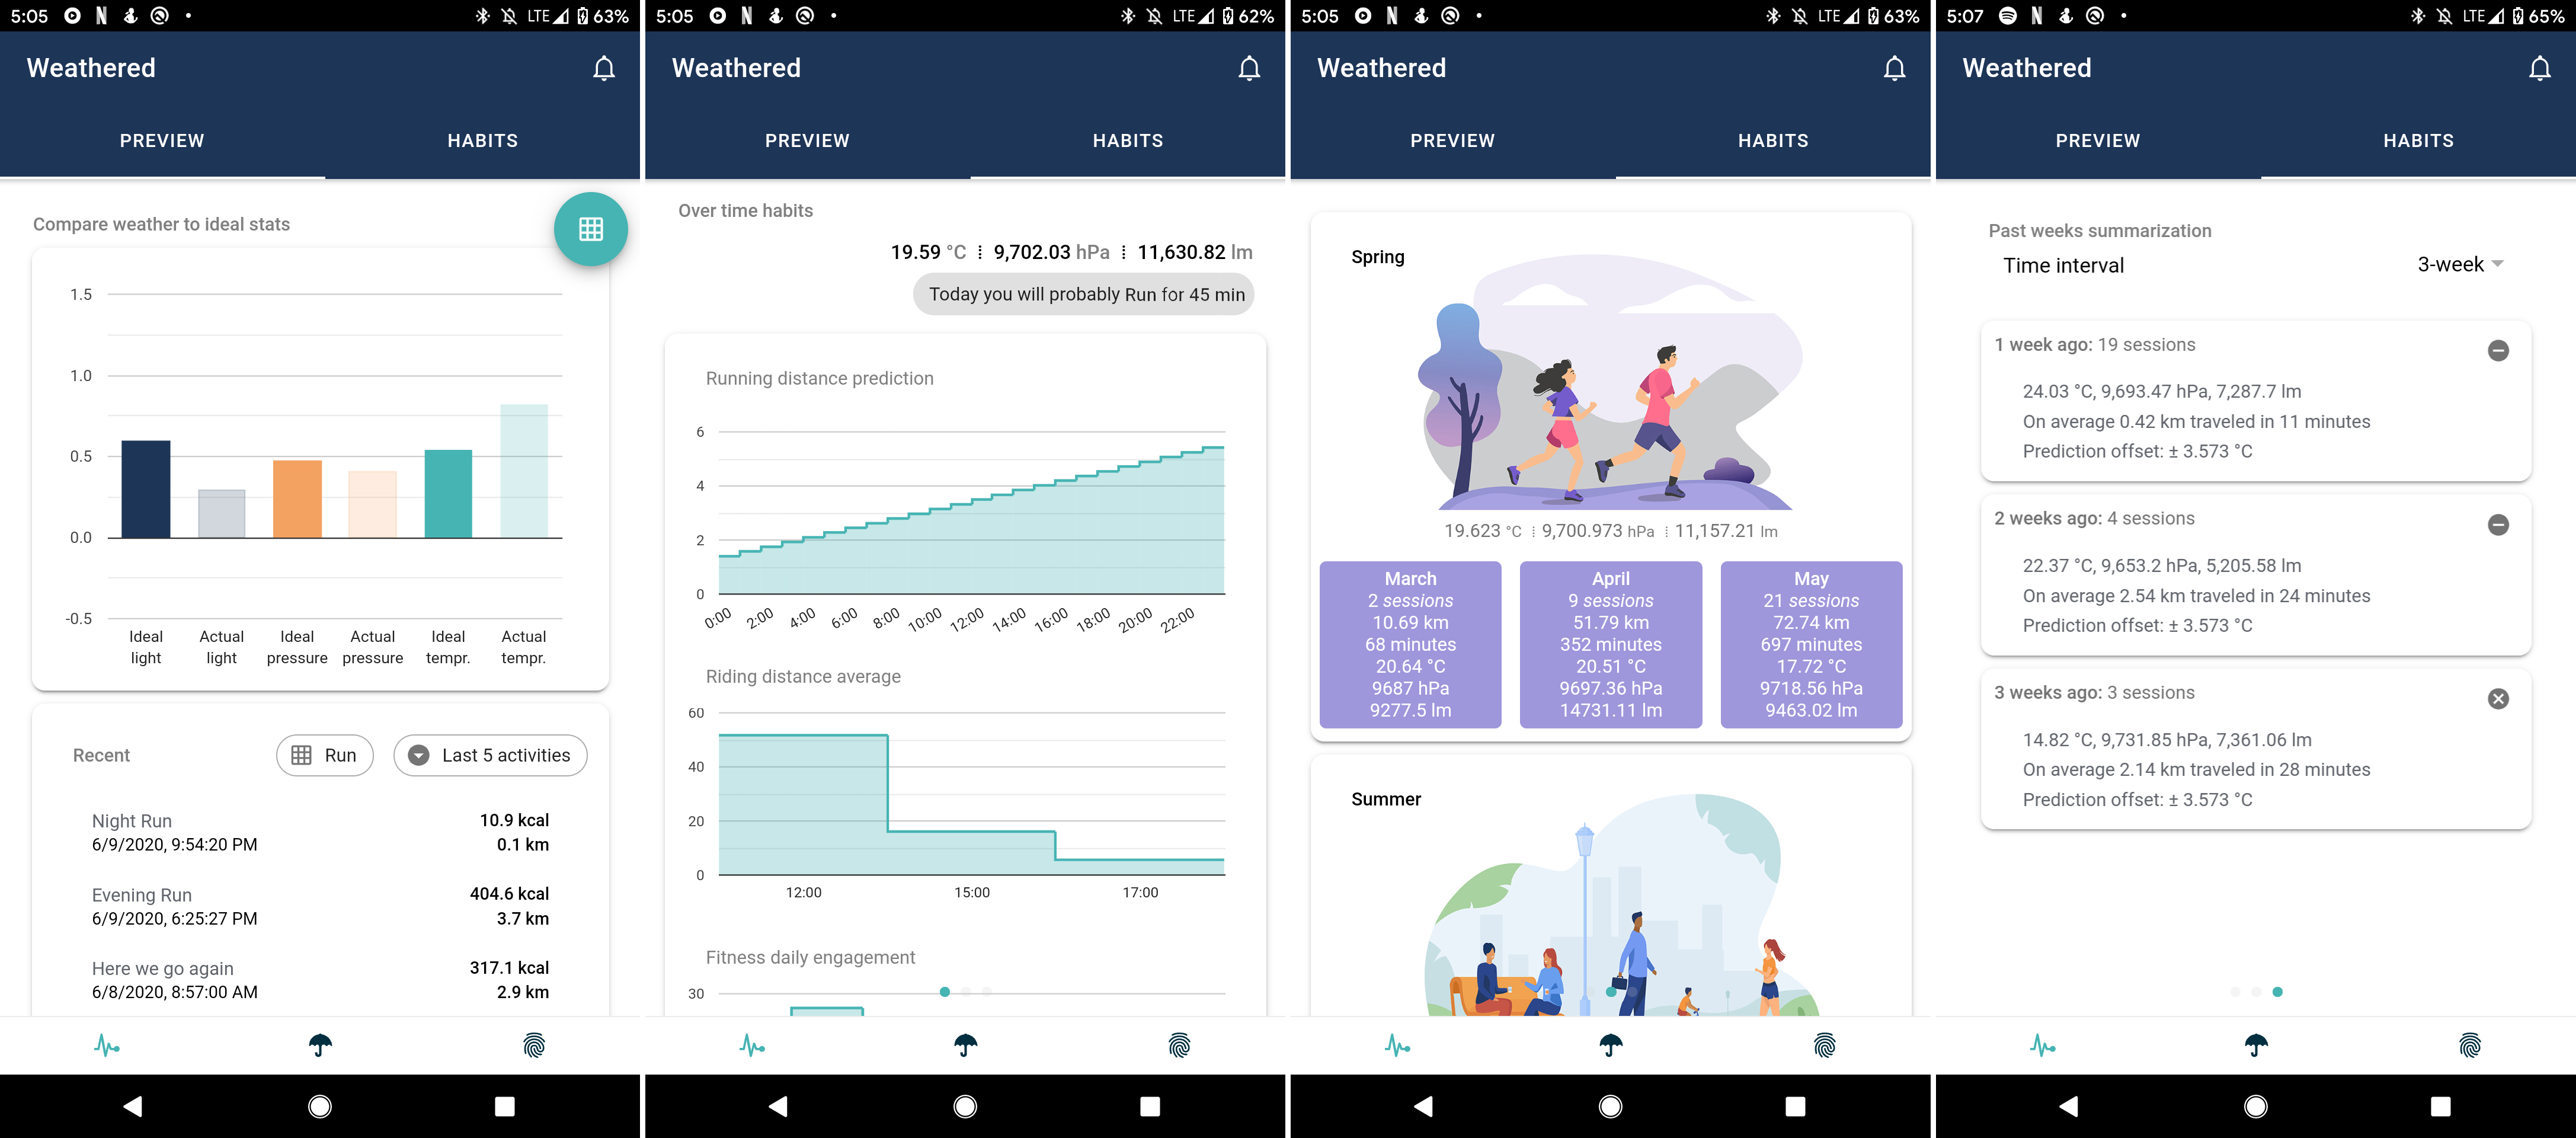
\includegraphics[width = 15.5cm]{bachelor/figures/habits_panel}
    \caption{Fitness habits panel}
    \label{fig:fitness_habits_panel}
\end{figure}

\subsection{Real-time weather measurements}

The weather monitor panel allows the user to check the current data, have a better understanding of the last 24 hours, change the display settings on the physical device and pair/un-pair a weather device. For the moment, only one weather device exists, and it is opened and closed manually, so that by pairing a device, the reader must understand that we can decide, for example, to save electrical energy by closing the communication channel between the weather monitor and the mobile application. In order to maintain a constant connection or stop data streaming between the mobile application and the weather device, one can use the upper-right corner button to navigate to the "Connected device" panel.

In the top-left side, the "Measurements" label is followed by a down-arrow button that makes the available measurement options visible when clicked. From left to right, selecting one of them adapts the current display to present the following: temperature, air pressure, ambient light, ambient color and the normalized values for temperature, air pressure and ambient light. Each measurements display has a real time component, a overview of the last 24 hours and two display options. Selecting one point of the graph offers a detailed overview of a specific point. Given that sometimes we deal with unexpected errors, and the user must know that an error occurred, a notification will appear on the screen.

\begin{figure}[!htb]
    \centering
    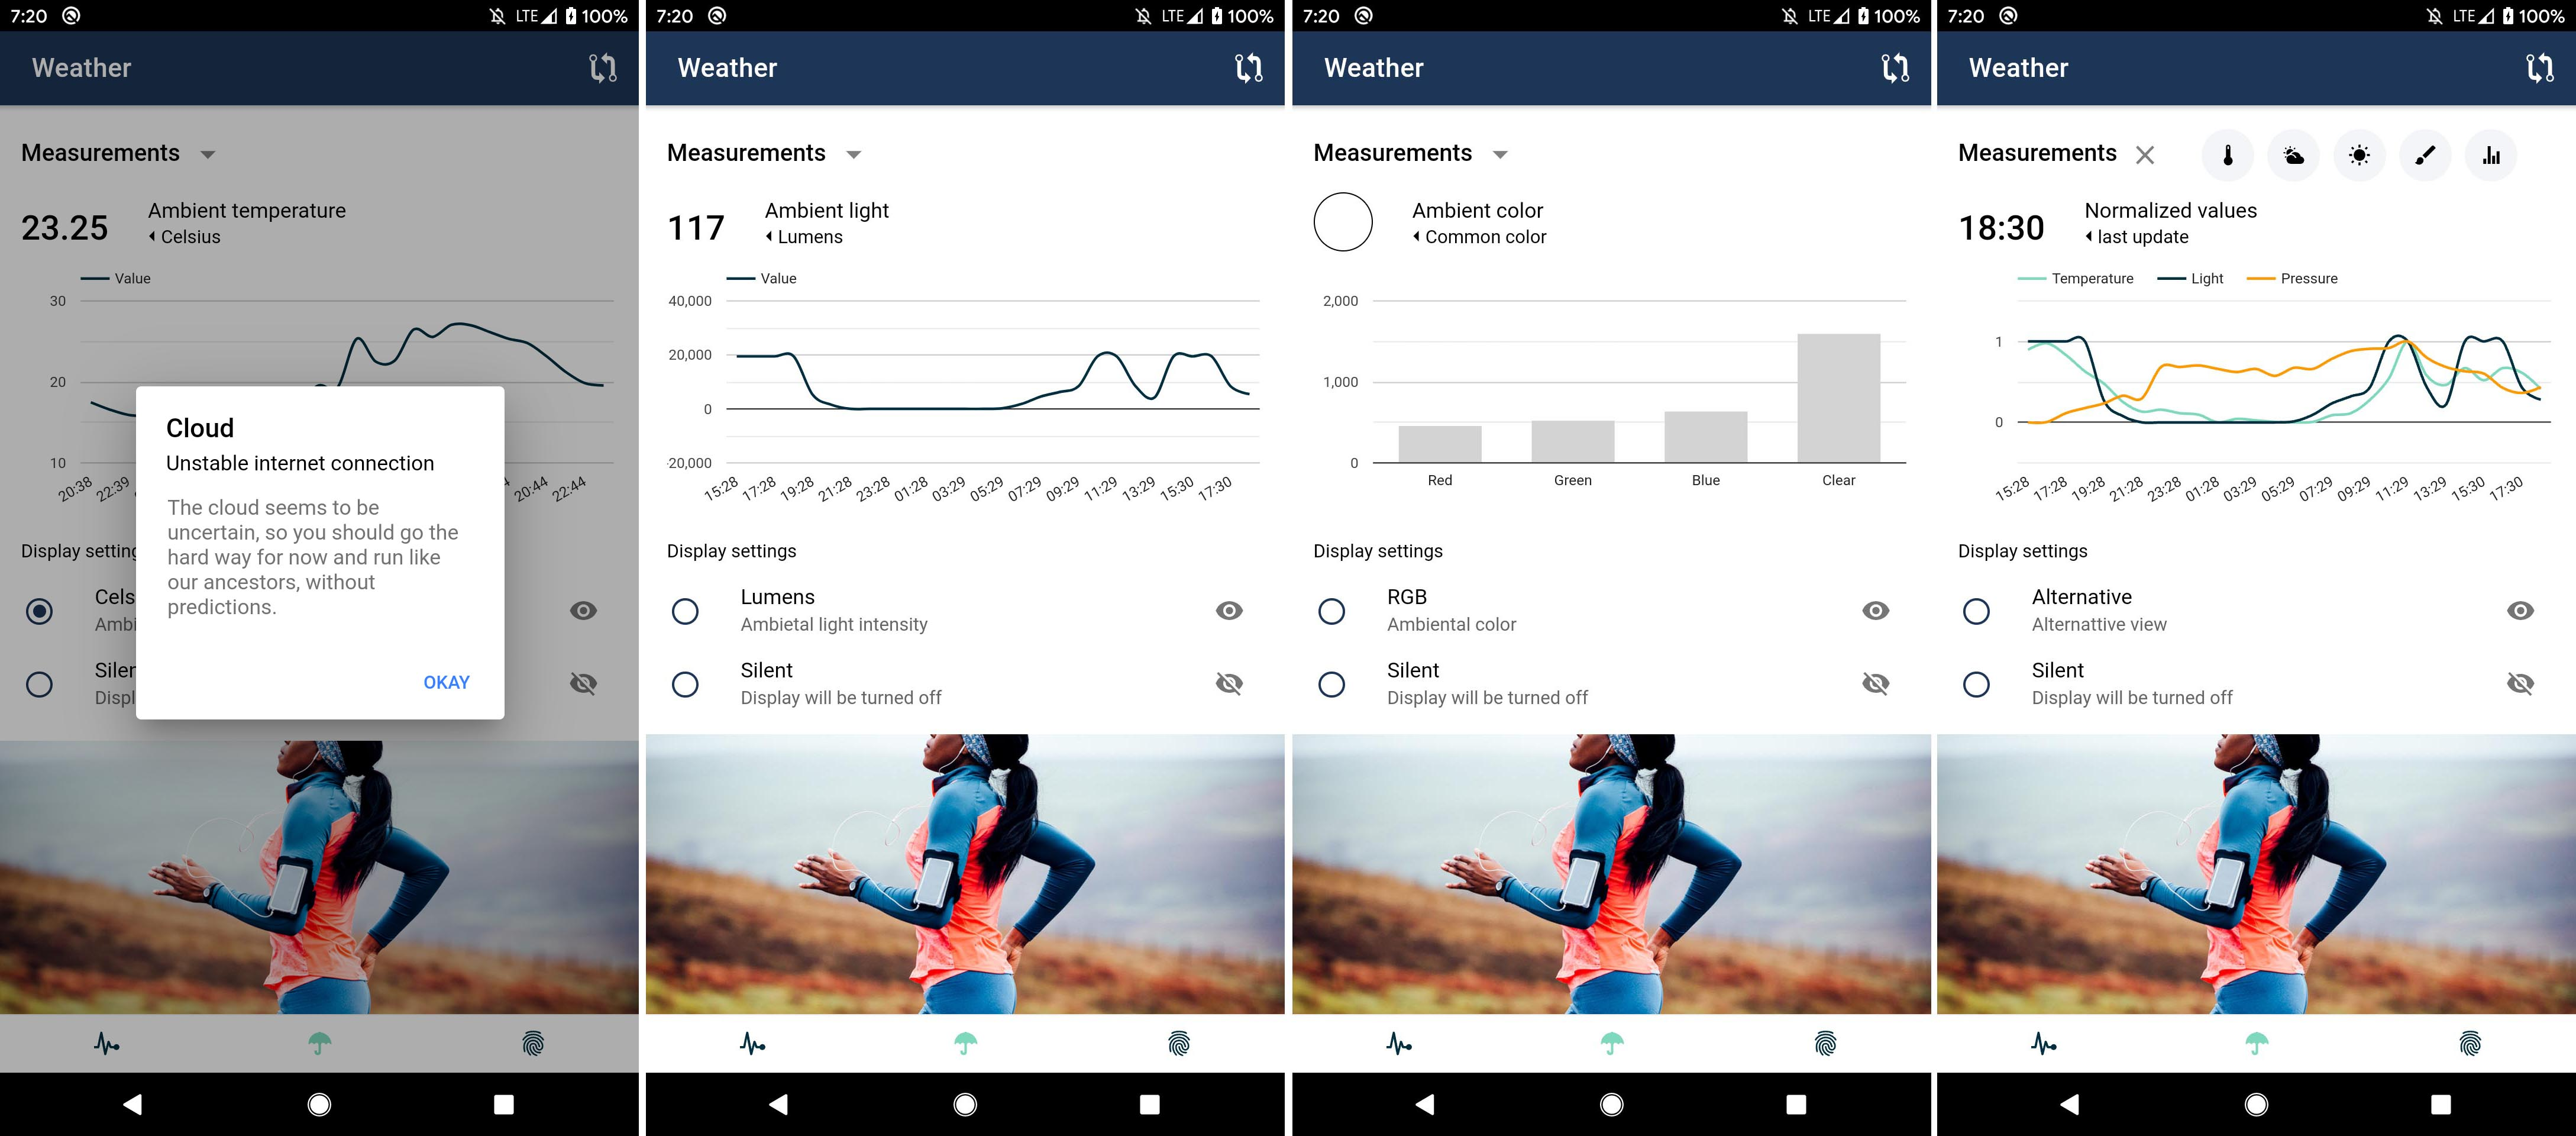
\includegraphics[width = 15.5cm]{figures/monitor_view}
    \caption{Real-time weather measurements panel}
    \label{fig:real_time_weather_measurements_panel}
\end{figure}

There are \textbf{four display options} one can select from the app menu: \textbf{only} the temperature, air pressure or light, those mention above in an \textbf{alternative} fashion, one for the color, and finally, a \textbf{silent} display option. The color was a great addition to the project, yet it is hard to actually see color shades, ones that are not easy to distinct. This feature can be replaced in future versions or improved, yet it is something that encourages a creative view on the project, so it was kept as it is right now. A better design can bring value by making the monitor glow in the same color palette with the environment.

\subsection{Fitness tracker statistics}

Last but not least, the fitness tracker panel is a direct overview of the athlete's activities. They were taken from Strava API and reshaped so that they fit the allure of this application. The complete documentation can be found at \url{https://developers.strava.com/docs/reference/}. The information is color coded, and labeled on columns so that a potential user can see the corresponding activity type for each row of information. There are multiple sports that were intentionally omitted and can be integrated in future versions, yet they were not adding any value to the current stage of the application. As an assumption, a survey must be conducted in order to better understand what is important to a user, or a user interface or design team can make it incorporate more information in less visuals. 

Using the upper-right corner button, one can sync its Strava account with the application. Selecting the sync option will open the authentication process which is handled by Strava. Gaining better understanding on the people and the business side this project might have one day, also leads to a better understanding of a proper log in, register and sync operations. As for this moment in time, they cannot be tailed to fit this application.
\begin{figure}[!htb]
    \centering
    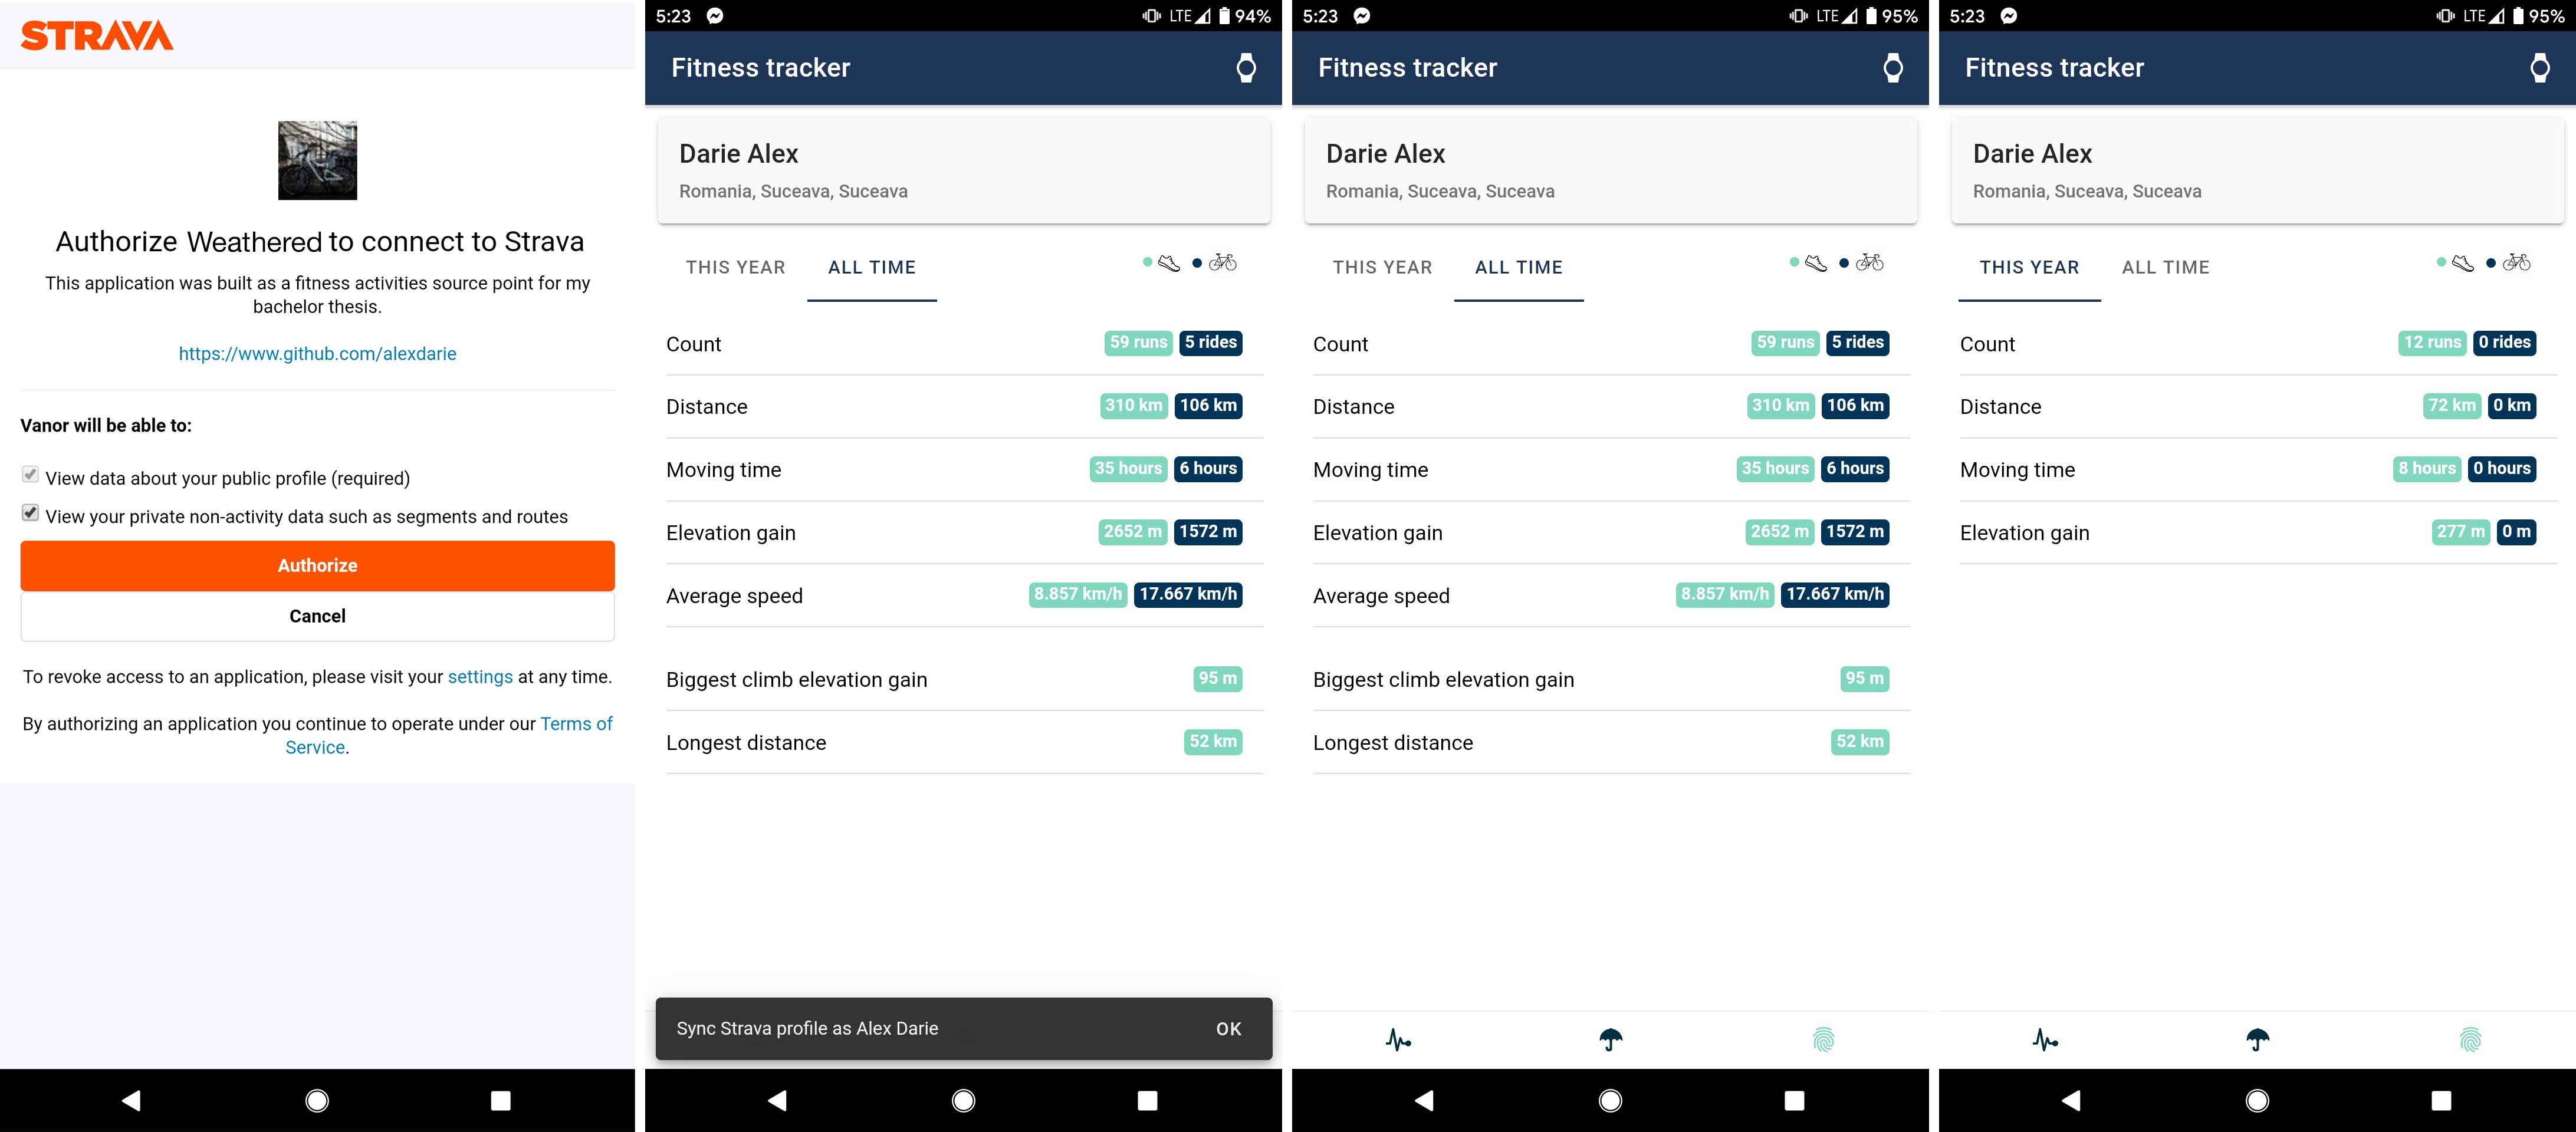
\includegraphics[width = 15.5cm]{figures/stats_panel}
    \caption{Fitness statistics panel}
    \label{fig:fitness_statistics_panel}
\end{figure}

